\h{Comparative Analysis}

\begin{refsection}[references/0001_6_other_theories.bib]

Energetically Coherent Computation (ECC) exists in complex dialogue with established theories of consciousness, offering both convergences and significant departures. The framework provides a distinctive physical grounding that reshapes our conceptualization of conscious experience while engaging with key insights from major theoretical approaches.

The relationship between ECC and Integrated Information Theory (IIT) proves particularly instructive. Where IIT posits that consciousness emerges from integrated information with high $\Phi$ values \cite{Koch2018}, ECC suggests consciousness arises from coherent energy flows within physical substrates. While both theories emphasize unity and integration, they propose fundamentally different mechanisms. IIT focuses on abstract information integration independent of physical substrate, while ECC emphasizes physically grounded energy dynamics and coherence patterns. This distinction carries significant implications for artificial consciousness - while IIT suggests consciousness could emerge in any system with sufficient information integration, ECC requires specific physical conditions and energy dynamics.

Global Workspace Theory (GWT) similarly finds both resonance and tension with ECC. While GWT describes consciousness as information gaining access to a "global workspace" for widespread broadcasting \cite{Baars2019}, ECC frames consciousness as emerging from coherent energy fields. Where GWT focuses on information access and distribution, ECC examines the underlying field dynamics that enable global integration. This shifts the emphasis from discrete broadcasting to continuous coherence maintenance.

Higher Order Theories (HOT) posit that consciousness requires higher-order representations of mental states \cite{Block2020}. ECC contrasts sharply with this view by suggesting consciousness emerges directly from coherent energy dynamics. Rather than requiring meta-representations, ECC grounds consciousness in base-level energy coherence. This reflects a fundamental difference in how the theories conceptualize the architecture of conscious experience.

The predictive processing framework finds interesting parallel developments with ECC, though through different mechanisms \cite{Clark2019}. While predictive processing uses abstract Bayesian inference hierarchies, ECC examines concrete energy dynamics. Both theories emphasize self-organization, but ECC grounds this organization in physical energy flows rather than abstract prediction error minimization \cite{Friston2020}.

This comparative analysis reveals ECC as offering a distinct perspective that emphasizes physical grounding while engaging with key insights from other theories. By examining how patterns of energetic coherence relate to established theoretical frameworks, ECC suggests new ways to understand both the possibilities and limitations of conscious systems. The framework's emphasis on physical grounding opens new avenues for empirical investigation while maintaining productive dialogue with existing theoretical approaches.

A fundamental distinction emerges when examining how most theories of consciousness tacitly adopt computationalist assumptions \cite{Chalmers2018}. Even theories that seem to move beyond pure computation - like IIT or GWT - often retain an underlying commitment to treating consciousness as fundamentally computational. ECC breaks from this tradition by suggesting that consciousness emerges from physical energy dynamics that cannot be reduced to computation alone.

The fundamental distinctions between various theories of consciousness become particularly evident when examining their treatment of empirical findings. Global Workspace Theory describes consciousness through the metaphor of a computational theater where different processors compete for access \cite{Baars2019}. While this model captures important aspects of conscious access, it remains fundamentally computational in its architecture. ECC suggests instead that what appears as competition for conscious access actually reflects competition between different patterns of energetic coherence, grounded in physical rather than computational dynamics.

Similarly, predictive processing frameworks typically describe hierarchical prediction using the language of Bayesian computation, even when emphasizing embodied aspects of cognition \cite{Clark2019}. ECC reconceptualizes prediction not as computational Bayesian inference but as emerging from stable patterns of energetic coherence that naturally anticipate future states through their physical dynamics. This shifts the theoretical foundation from abstract probability distributions to concrete energy flows \cite{Friston2020}.

Higher Order Theories, despite moving beyond simple computation by introducing meta-representational requirements \cite{Block2020}, still generally assume these representations operate through computational mechanisms. ECC suggests instead that any metacognitive capacities emerge from specific patterns of energetic coherence rather than computational hierarchies. This grounds higher-order awareness in physical dynamics rather than abstract computation.

Even Integrated Information Theory, while breaking important ground in linking consciousness to physical systems \cite{Koch2018}, retains computational assumptions in how it quantifies integration through mathematical information theory. ECC suggests that integration emerges not from abstract information processing but from actual patterns of energetic coherence maintained through biological mechanisms \cite{Tononi2021}.

The persistence of computationalist assumptions across theories of consciousness reflects the powerful influence of the computational metaphor in cognitive science. However, this reliance on computation may ultimately limit our understanding of consciousness. ECC suggests that consciousness requires specific forms of physical organization that cannot be captured through computational models alone \cite{Dehaene2021}.

This insight carries significant implications for artificial consciousness. Where computationalist theories suggest consciousness could emerge from sufficient computational complexity, ECC indicates that conscious machines would require specific physical architectures capable of maintaining coherent energy dynamics similar to biological systems. This provides clearer constraints on what types of systems could potentially support consciousness while suggesting new directions for artificial consciousness research beyond traditional computational approaches.

By grounding consciousness in energetic coherence rather than computation, ECC offers a framework for understanding features of conscious experience that prove difficult to explain computationally - from the unity of consciousness to the qualitative richness of experience \cite{Lamme2020}. This suggests that progress in understanding consciousness may require moving beyond computational paradigms to examine the underlying physical dynamics that make conscious experience possible.

This theoretical reframing helps resolve longstanding philosophical issues like the symbol grounding problem more directly. Rather than attempting to connect abstract symbols to meaning through computational processes, ECC suggests how meaning emerges naturally from patterns of energetic coherence grounded in physical reality. This provides a more fundamental basis for understanding how conscious systems achieve genuine intentionality and semantic content \cite{Chalmers2018}.

The embodied and phenomenological dimensions of consciousness take on particular significance when examined through ECC's framework. While traditional cognitive science often treats embodiment as an implementation detail, the enactive approach developed in foundational work emphasizes how consciousness emerges from the dynamic coupling between organism and environment \cite{Varela2017}. ECC strengthens this perspective by providing concrete physical mechanisms through which such coupling occurs via patterns of energetic coherence.

The relationship between consciousness and biological processes finds sophisticated treatment in recent theoretical developments \cite{Thompson2018}. Rather than treating biological implementation as incidental to conscious processing, ECC suggests that specific biological mechanisms enable the particular forms of energetic coherence necessary for consciousness. This aligns with emerging perspectives that emphasize the deep continuity between life and mind while providing physical mechanisms to explain this connection.

Recent work on the predictive aspects of conscious experience has suggested important links between perception, action, and conscious awareness \cite{Seth2021}. ECC reframes these predictive relationships not as computational processes but as emerging naturally from the physical dynamics of coherent energy fields. This provides a more fundamental basis for understanding how conscious systems achieve the anticipatory capabilities emphasized in contemporary theories.

The electromagnetic field theory of consciousness offers interesting parallels with ECC's framework \cite{McFadden2020}. While both approaches emphasize field-like properties of conscious experience, ECC suggests that electromagnetic fields represent just one aspect of the broader patterns of energetic coherence necessary for consciousness. This more comprehensive view helps explain how different physical mechanisms integrate to create unified conscious experience.

Higher-order theories of consciousness have proposed sophisticated models of how self-awareness emerges through metacognitive representation \cite{Rosenthal2019}. ECC suggests instead that self-awareness emerges naturally from recursive patterns of energetic coherence without requiring explicit meta-representation. This provides a more parsimonious account of how conscious systems achieve self-awareness while maintaining closer contact with physical dynamics.

This synthesis reveals ECC as offering a distinctive theoretical framework that engages productively with existing theories while suggesting new directions for consciousness research. By grounding conscious experience in patterns of energetic coherence rather than abstract computation or pure phenomenology, ECC provides concrete mechanisms that help bridge traditional divides between physical and experiential approaches to consciousness. This theoretical integration suggests promising directions for future empirical investigation while maintaining rigorous connection to both physical and phenomenological aspects of conscious experience.
     
\section{IIT and Panpsychism}

%TODO: this section is quite repetitive

The relationship between Energetically Coherent Computation (ECC) and both Integrated Information Theory (IIT) and panpsychist approaches reveals important theoretical convergences while maintaining distinct positions on consciousness's physical basis. Where IIT posits consciousness as identical to integrated information \cite{Tononi2008}, and panpsychism suggests consciousness pervades all matter \cite{Strawson2006}, ECC frames consciousness as emerging from specific patterns of energetic coherence within biological systems.

At its core, IIT offers a mathematical framework for quantifying consciousness through integrated information ($\Phi$) \cite{Tononi2016}. While ECC appreciates IIT's attempt to provide rigorous measures of consciousness, it suggests that integration emerges from physical energy dynamics rather than abstract information processing. This distinction proves crucial - where IIT remains largely substrate-independent, ECC insists on specific physical requirements through energetic coherence and field dynamics. The rich alphabet requirement in ECC, shaped by transcriptomic profiles and cellular organization, provides concrete constraints on possible implementations of consciousness that go beyond IIT's more abstract specifications.

ECC aligns with panpsychism in rejecting purely computational approaches to consciousness and emphasizing its grounding in physical reality \cite{Nagel1979}. However, where panpsychism attributes consciousness to all matter, ECC suggests consciousness requires specific forms of energetic coherence typically found only in biological systems. This more restricted view helps avoid the combination problem that plagues panpsychist accounts \cite{Chalmers2015} - how simple forms of consciousness combine into complex experiences. ECC explains this through its framework of coherent energy dynamics and field integration.

The theories also differ in their treatment of emergence \cite{Goff2019}. Panpsychism often posits consciousness as fundamental, while IIT suggests it emerges from information integration \cite{Oizumi2014}. ECC charts a middle path, proposing that consciousness emerges from specific patterns of energetic coherence while remaining irreducibly physical. This approach maintains connection to physical reality while explaining why consciousness appears only in certain types of organized systems.

Particularly significant is how ECC addresses the explanatory gap between physical processes and conscious experience \cite{Koch2019}. Rather than making consciousness ubiquitous like panpsychism or reducing it to information like IIT, ECC suggests how specific patterns of energetic coherence give rise to conscious experiences through their inherent physical dynamics. This provides a more concrete basis for understanding both the emergence of consciousness and its qualitative features.

The historical development of panpsychist thought in Western philosophy \cite{Skrbina2017} reveals persistent tensions that ECC's framework helps address. While panpsychism attempts to solve the hard problem by making consciousness fundamental to all matter, and IIT seeks to bridge the explanatory gap through information theory \cite{Tononi2015}, ECC suggests that the qualitative aspects of consciousness emerge naturally from specific patterns of energetic coherence, providing a physical basis for phenomenal experience without reducing it to computation or making it universal.

This theoretical synthesis suggests ECC might help bridge aspects of IIT and panpsychism while maintaining its distinctive emphasis on physical energy dynamics. By grounding consciousness in specific patterns of energetic coherence, ECC provides a framework that acknowledges both the physical basis of consciousness and its emergence in complex biological systems, while avoiding the metaphysical challenges that have historically plagued both panpsychist and purely informational approaches \cite{Shani2015}.

The dynamic core hypothesis, developed before IIT, provides an important historical bridge between neural integration theories and ECC's framework. Where the dynamic core hypothesis proposed that consciousness emerges from integrated neural activity in thalamocortical systems, ECC extends this insight by specifying how such integration occurs through coherent energy dynamics. Both approaches emphasize the importance of dynamic integration \cite{Tononi2008}, but ECC grounds this integration in physical field effects rather than purely neural computation.

Particularly relevant is how the dynamic core hypothesis identified the importance of rapid neural integration and differentiation. ECC builds on this insight by explaining how such integration occurs through field-like properties of energetic coherence, maintained through astrocytic networks and the extracellular matrix. This provides a physical mechanism for the kind of dynamic integration that early IIT described primarily in computational terms \cite{Oizumi2014}.

The progression from dynamic core to IIT to ECC reveals an interesting theoretical evolution. The dynamic core hypothesis began with biological neural systems, IIT abstracted these principles into substrate-independent information integration \cite{Tononi2015}, and ECC returns to physical implementation while maintaining mathematical rigor through its sheaf-theoretic framework and stress-energy tensor formalism.

This theoretical progression also illuminates key differences in how these frameworks approach the hard problem of consciousness \cite{Chalmers2015}. Panpsychism attempts to dissolve the hard problem by making consciousness fundamental to all matter \cite{Strawson2006}. IIT seeks to bridge the explanatory gap through information theory. ECC suggests instead that the qualitative aspects of consciousness emerge naturally from specific patterns of energetic coherence, providing a physical basis for phenomenal experience without reducing it to computation or making it universal.

The relationship between these theories has important implications for understanding both biological and artificial consciousness \cite{Koch2019}. Where IIT opened the possibility of non-biological consciousness through information integration, ECC suggests more specific requirements based on energetic coherence. This provides clearer constraints on what types of systems could potentially support consciousness while explaining why biological systems prove particularly suited to generating conscious experience.

These theoretical relationships also help clarify how consciousness might have evolved \cite{Goff2019}. Rather than consciousness being either fundamental (panpsychism) or emerging suddenly through sufficient information integration (IIT), ECC suggests a gradual evolution of increasingly sophisticated patterns of energetic coherence in biological systems. This aligns with recent research in cellular cognition and basal awareness while explaining how more complex forms of consciousness emerged \cite{Mathews2011}.

IIT's relationship to panpsychism emerges from its fundamental premise that consciousness is identical to integrated information \cite{Tononi2016}. Since information integration exists to some degree in all physical systems, IIT leads naturally toward a panpsychist view where consciousness exists ubiquitously, though in varying degrees. This marks a crucial difference from ECC, which identifies consciousness with specific patterns of energetic coherence rather than information integration per se.

This tendency toward panpsychism represents both a strength and limitation of IIT \cite{Tononi2008}. While it provides a unified theoretical framework, it struggles to explain why consciousness appears limited to certain types of systems and how simple forms of consciousness combine into complex experiences \cite{Chalmers2015}. ECC addresses these challenges by specifying physical requirements for consciousness through energetic coherence, transcriptomic profiles, and field dynamics.

The progression from early work on the dynamic core to IIT's more abstract formulation reveals an interesting theoretical trajectory \cite{Tononi2016}. Where the dynamic core hypothesis began with concrete neural mechanisms, IIT moved toward increasingly mathematical and substrate-independent descriptions. ECC suggests a return to physical implementation while maintaining mathematical rigor through its sheaf-theoretic framework and field dynamics.

Recent developments in panpsychist thought \cite{Skrbina2017} have attempted to address the combination problem through various theoretical innovations. However, these solutions often remain abstract and disconnected from biological reality. ECC's framework offers a more concrete approach by showing how physical patterns of energetic coherence naturally combine and integrate across scales without requiring additional metaphysical principles.

The cosmological implications of panpsychism \cite{Shani2015} raise important questions about the relationship between consciousness and fundamental physical processes. While ECC shares with panpsychism an emphasis on the physical basis of consciousness, it suggests that conscious experience requires specific forms of organized complexity rather than being inherent in all matter. This provides a clearer explanation for why consciousness appears in some systems but not others.

IIT's mathematical formalization of consciousness \cite{Oizumi2014} represents an important attempt to quantify conscious experience. However, its focus on information integration independent of physical implementation may miss crucial aspects of how consciousness actually emerges in biological systems. ECC maintains the mathematical rigor of IIT while grounding it more firmly in physical reality through its analysis of energetic coherence patterns.

The fundamental tension between panpsychist and emergentist approaches to consciousness \cite{Goff2019} finds potential resolution through ECC's framework. Rather than choosing between consciousness as fundamental or as purely emergent, ECC suggests how specific patterns of physical organization give rise to conscious experience through their inherent dynamics. This provides a middle path between panpsychist and emergentist extremes while maintaining clear connection to empirical investigation.

This theoretical synthesis suggests productive new directions for consciousness research that move beyond both pure computation and simple panpsychism \cite{Koch2019}. By examining how specific patterns of energetic coherence support conscious experience, we may develop more sophisticated understanding of both the physical basis of consciousness and its qualitative features. This approach maintains rigorous connection to physical reality while acknowledging the irreducible aspects of conscious experience that have motivated panpsychist approaches.

ECC and IIT share conceptual territory in their emphasis on integration as a fundamental property of conscious systems, though they differ markedly in their metaphysical commitments and explanatory frameworks \cite{Tononi2008}. 

A primary distinction lies in their treatment of physical implementation. ECC positions energy flows as foundational, viewing consciousness as emerging from coherent organization of energy across physical modalities - electromagnetic, chemical, and mechanical. This stands in contrast to IIT's more abstract approach, which, while acknowledging physical substrates, focuses primarily on informational integration and causal structures \cite{Tononi2016}. Where ECC rejects hardware-software distinctions as fundamental, IIT abstracts consciousness into mathematical frameworks independent of specific energetic dynamics.

The theories also diverge in their treatment of integration versus coherence. IIT defines consciousness through $\Phi$, a quantitative measure of integrated information that captures how irreducible a system's causal structure is to its constituent parts \cite{Oizumi2014}. ECC, conversely, emphasizes coherence grounded in energetic dynamics rather than pure information. This coherence encompasses energetic efficiency, field stability, and specific physical substrate requirements that extend beyond informational integration.

A further crucial distinction lies in their treatment of phenomenology. ECC positions phenomenal experience as directly emergent from physical energy patterns, while IIT approaches phenomenology through the mathematical quantification of integrated information \cite{Tononi2015}. This reflects a deeper philosophical divergence - where IIT maintains a degree of substrate independence that aligns with certain panpsychist interpretations \cite{Koch2019}, ECC insists on specific physical implementations that respect energetic coherence.

The ontological commitments of these frameworks reveal fundamentally different approaches to consciousness. IIT's mathematical formalization of consciousness as integrated information suggests alignment with broader panpsychist traditions \cite{Chalmers2015}, while ECC's insistence on specific physical dynamics positions it closer to biological naturalism. These distinct metaphysical foundations shape how each theory approaches key questions in consciousness research, from the hard problem to the possibility of machine consciousness.

This analysis reveals not just theoretical differences but fundamentally distinct research programs. Where IIT directs attention toward mathematical formalization of information integration, ECC emphasizes investigation of physical energy dynamics in biological systems. These divergent approaches suggest different experimental priorities and methodological commitments in consciousness research.

Through this comparative lens, we see how ECC and IIT represent distinct paradigms in consciousness research, each offering unique insights while maintaining different relationships to the physical implementation of conscious experience. Their contrasting approaches to physical substrates, integration, and phenomenology illuminate crucial questions about the nature of consciousness and its relationship to physical reality.

The ontological distinctions between ECC and IIT reflect broader debates in consciousness studies about the relationship between physical implementation and mental phenomena \cite{Nagel1979}. Where ECC grounds consciousness in physical energy dynamics, IIT's more abstract informational framework aligns with certain strands of computational theory of mind while maintaining unique metaphysical commitments \cite{Tononi2016}.

ECC's physicalist ontology positions energy flows as the fundamental constituents of both physical reality and consciousness. This approach emphasizes direct causation through electromagnetic, chemical, and thermal dynamics, rejecting abstractions that separate computational description from physical implementation. The theory suggests that specific perturbations in energy flows correspond directly to changes in phenomenal experience, making concrete predictions about the relationship between physical dynamics and conscious states \cite{Koch2019}.

In contrast, IIT operates from an informational ontology where consciousness emerges from specific patterns of integrated information, quantified through $\Phi$ \cite{Oizumi2014}. This framework treats information structures and their causal relationships as primary, allowing for substrate independence in principle. While acknowledging the need for physical implementation, IIT positions the mathematical structure of information integration as the essential feature of consciousness.

These distinct ontological commitments shape how each theory approaches the relationship between brain and consciousness. ECC's emphasis on specific physical dynamics aligns with certain aspects of naturalistic approaches \cite{Goff2019}, while suggesting that consciousness requires particular forms of energetic coherence that cannot be reduced to abstract computation. IIT's more abstract framework, while mathematically sophisticated, raises questions about the relationship between information, causation, and physical implementation \cite{Tononi2015}.

The theories' divergent approaches to substrate independence particularly illuminate their philosophical differences. ECC's insistence on specific physical implementation suggests that consciousness cannot be realized in arbitrary substrates, even if they implement similar computational structures. This contrasts with IIT's more permissive view regarding physical implementation, though both theories maintain sophisticated accounts of how consciousness relates to physical systems \cite{Strawson2006}.

These ontological distinctions carry significant implications for consciousness research. ECC directs attention toward investigating specific physical mechanisms and energy dynamics in biological systems, while IIT emphasizes mathematical modeling of information integration. Both approaches contribute valuable insights while suggesting different experimental priorities and methodological commitments in the study of consciousness.

The contrast between energetic and informational ontologies also raises important questions about the nature of causation in conscious systems. ECC's emphasis on physical energy flows suggests direct causal relationships between neural dynamics and conscious experience, while IIT's focus on informational integration provides a different perspective on mental causation \cite{Tononi2008}. These different approaches to causation reflect broader philosophical debates about the relationship between physical and mental phenomena.

Through careful examination of these ontological commitments, we gain deeper insight into how different theoretical frameworks approach the challenge of explaining consciousness. The contrast between ECC and IIT illuminates crucial questions about the relationship between physical implementation, information processing, and conscious experience.

The philosophical implications of these contrasting frameworks extend beyond theoretical distinctions to fundamental questions about the nature of consciousness and its place in physical reality \cite{Skrbina2017}. ECC's energetic monism suggests a unified view where energy serves as the foundational substance underlying both physical and phenomenal properties. This perspective aligns with certain naturalistic approaches while maintaining distinct claims about the specific physical requirements for consciousness.

IIT's framework, in contrast, suggests what might be termed an informational dual-aspect theory, where information possesses both physical and experiential aspects \cite{Tononi2016}. This approach shares certain features with panpsychist perspectives while maintaining its unique emphasis on integrated information as the basis for consciousness \cite{Mathews2011}. The theory's mathematical formalization of consciousness through $\Phi$ suggests a kind of pan-computationalism, though with specific requirements for information integration that distinguish it from simpler computational theories.

These distinct philosophical commitments shape how each theory approaches key questions in consciousness research. ECC's emphasis on physical dynamics suggests that understanding consciousness requires detailed investigation of energy flows in biological systems, particularly focusing on electromagnetic fields and chemical gradients in neural tissue. IIT, conversely, directs attention toward developing increasingly sophisticated mathematical models of information integration \cite{Oizumi2014}.

The theories also differ in their predictions about artificial consciousness. ECC's insistence on specific physical implementation suggests strict constraints on what types of systems could potentially support consciousness, requiring particular forms of energetic coherence typically found in biological systems. IIT's more abstract framework allows for the possibility of conscious artificial systems, provided they achieve sufficient levels of integrated information \cite{Koch2019}.

The relationship between phenomenology and physical implementation represents another crucial distinction. ECC suggests that conscious experience emerges directly from patterns of energetic coherence, making specific predictions about how physical perturbations should correspond to changes in phenomenal experience. IIT approaches phenomenology through mathematical formalization of information structures, suggesting different experimental approaches to investigating conscious experience \cite{Shani2015}.

These theoretical distinctions carry significant implications for the future of consciousness research. Where ECC suggests focusing on physical mechanisms and energy dynamics in biological systems, IIT points toward mathematical modeling and quantification of information integration. Both approaches offer valuable insights while maintaining different relationships to the hard problem of consciousness \cite{Goff2019}.

Through careful analysis of these theoretical frameworks, we gain deeper insight into the challenges and opportunities in consciousness research. The contrast between ECC and IIT illuminates crucial questions about the nature of consciousness, its relationship to physical reality, and the prospects for developing a comprehensive scientific understanding of conscious experience.

\begin{table}[h!]
\centering
\setlength{\extrarowheight}{2pt} % Adds extra row height for readability
\begin{tabularx}{\textwidth}{@{}p{3cm}Xp{4cm}@{}}
\toprule
\textbf{Aspect} & \textbf{ECC: Energy Ontology} & \textbf{IIT: Information Ontology} \\ \midrule
\textbf{Primary Basis} & Energy and its physical flows & Information and its causal structure \\
\textbf{Relation to Consciousness} & Arises from coherent energy flows across physical modalities (e.g., electromagnetic, chemical) & Arises from integrated information ($\Phi$), quantified as the irreducibility of causal interactions \\
\textbf{Role of Physicality} & Physical energy flows are fundamental; no abstraction between hardware and software & Physical implementation is secondary; causal informational structure is primary \\
\textbf{Phenomenology} & Grounded in energy patterns and their dynamic organization; directly tied to physical energy flows & Grounded in abstract informational integration; explained through the mathematical structure of $\Phi$ \\
\textbf{Substrate Dependence} & Substrate-specific: requires physical systems capable of coherent energy organization (e.g., EM fields in neurons) & Substrate-independent: any system with sufficient integrated causal structures \\
\textbf{Core Mechanism} & Coherence of energy dynamics enabling integration and efficiency in physical systems & Irreducible integration of information as measured by $\Phi$ \\
\textbf{Richness of Representation} & Based on a rich alphabet of energy flows (e.g., electromagnetic, chemical) to form high-dimensional states & Based on binary or abstract informational states, emphasizing causal interaction \\
\textbf{Research Direction} & Physical energy dynamics in the brain (e.g., EM fields and ion flows) & Models of informational integration and causal structures \\
\textbf{Philosophical Alignment} & Energetic monism: energy as the unifying substance of conscious and physical phenomena & Dual-aspect theory or pancomputationalism: information as the fundamental basis for consciousness \\ \bottomrule
\end{tabularx}
\caption{Energetically Coherent Computation (ECC) and Integrated Information Theory (IIT)}
\label{tab:ecc_vs_iit}
\end{table}

\section{Global Workspace Theory}

Bernard Baars' Global Workspace Theory (GWT) portrays consciousness as a kind of theater where multiple parallel processes compete for access to a limited-capacity global workspace. Once information gains access to this workspace, it becomes globally available to diverse brain regions through a process of broadcasting \cite{Baars1988}. This metaphor has proven remarkably productive for cognitive science and neuroscience research, generating numerous experimental predictions and therapeutic applications \cite{Dehaene2001}.

ECC shares with GWT the recognition that consciousness involves a form of integration and broadcast across brain regions \cite{Baars2002}. However, where GWT describes this process primarily in terms of information flow and access, ECC grounds it in physical energy dynamics and coherent fields. The "broadcast" in ECC isn't the transmission of abstract information but rather the achievement and maintenance of energetic coherence across neural tissues.

The limited capacity of consciousness, which GWT explains through workspace constraints \cite{Dehaene2006}, finds a different interpretation in ECC through the concept of energetic coherence and neural light cones. The brain can only maintain coherent energy states across a limited domain, constrained by physical and thermodynamic factors. This provides a physical basis for the capacity limitations that GWT describes in more abstract terms.

Competition for conscious access, a central feature of GWT \cite{Dehaene2011}, takes on new meaning within ECC's framework. Rather than competing for entry into an abstract workspace, neural processes compete to achieve and maintain coherent energy states within the brain's physical architecture. This competition is governed by thermodynamic constraints and the requirements for maintaining stable, low-entropy configurations across neural tissues.

Recent developments in GWT have emphasized the role of cortical binding and propagation in enabling conscious contents \cite{Baars2013}. ECC's emphasis on transcriptomic profiles and molecular dynamics extends this framework by suggesting how different brain regions might be differentially equipped to participate in conscious processing. The "rich alphabet" of possible states in different brain regions, shaped by their specific molecular characteristics, influences how they can contribute to the coherent field of consciousness.

Where GWT describes consciousness primarily through information processing and access consciousness \cite{Dehaene2014}, ECC suggests that even phenomenal consciousness - the raw feel of experience - emerges from specific patterns of energetic coherence. This offers a potential bridge between access and phenomenal consciousness, grounding both in physical energy dynamics rather than abstract information processing \cite{Mashour2020}.

The theoretical framework of GWT has been significantly advanced through mathematical treatments \cite{Wallace2005} and computational modeling \cite{Franklin1999}. However, ECC suggests that these formal approaches, while valuable, may miss crucial aspects of how consciousness emerges from physical dynamics rather than computational processes. Future research might productively explore how GWT's insights about information broadcast could be integrated with ECC's emphasis on energy dynamics.

The contrast between GWT's broadcast architecture and ECC's field dynamics raises fundamental questions about the temporal structure of consciousness \cite{Sergent2004}. Where GWT suggests consciousness emerges through serial broadcasting of winning coalitions, ECC describes consciousness as continuous patterns of energetic coherence that maintain stability through recursive feedback. This temporal aspect becomes particularly significant when considering how different brain regions achieve coordinated activity.

Recent work has expanded GWT by incorporating insights from network science and complex systems theory \cite{Shanahan2012}. While these developments provide sophisticated models of information flow in neural networks, ECC suggests that understanding consciousness requires examining how physical energy dynamics create and maintain coherent states across these networks. The brain's connective core may serve not just as an information hub but as a physical substrate for maintaining specific patterns of energetic coherence.

The neural mechanisms underlying global broadcasting have been extensively investigated \cite{Dehaene2014}, revealing how different brain regions coordinate to create conscious experience. ECC reframes these findings in terms of physical dynamics, suggesting that what appears as information broadcast may actually reflect the achievement and maintenance of specific patterns of energetic coherence across neural tissues \cite{Mashour2020}.

Contemporary versions of GWT have incorporated insights from predictive processing and hierarchical models \cite{Dehaene2011}, suggesting that conscious access involves both bottom-up and top-down processes. ECC provides a physical grounding for these interactions, showing how different scales of organization maintain coherent energy states through continuous feedback rather than discrete information exchange.

The relationship between attention and consciousness takes on particular significance in both frameworks \cite{Baars2013}. While GWT treats attention as a spotlight selecting content for conscious broadcast, ECC suggests that attentional effects emerge from modulations in patterns of energetic coherence. This provides a more fundamental physical basis for understanding how attention shapes conscious experience.

The experimental evidence supporting GWT \cite{Sergent2004} remains valuable while suggesting new interpretations through ECC's framework. Phenomena like the attentional blink and conscious access thresholds may reflect constraints on maintaining coherent energy states rather than limitations of an abstract workspace. This reframing helps bridge theoretical models with biological mechanisms.

Through this lens, consciousness emerges not just as a workspace for information sharing but as a physically grounded field of coherent energy dynamics, constrained by biological structure and thermodynamic principles \cite{Dehaene2001}. This perspective enriches GWT while maintaining its valuable insights about the integrative nature of conscious experience.

The empirical support for GWT has grown substantially through neuroimaging studies and cognitive experiments \cite{Dehaene2006}. While these findings are often interpreted through an information processing lens, ECC suggests they might better be understood as revealing how different brain regions achieve and maintain coherent energy states. This reinterpretation preserves the empirical insights while grounding them more firmly in physical dynamics.

Recent theoretical developments have expanded GWT to address questions of cognitive architecture and neural implementation \cite{Mashour2020}. While these models have become increasingly sophisticated in their treatment of information flow and neural dynamics, ECC suggests that understanding consciousness requires examining how physical energy patterns create and maintain coherent states across neural tissues. The global workspace may represent not just an information-sharing network but a physically realized field of coherent energy dynamics.

The relationship between conscious and unconscious processing, a central concern in GWT \cite{Dehaene2011}, finds new expression through ECC's framework. Rather than focusing on access to a broadcast mechanism, ECC suggests that the conscious-unconscious distinction reflects different patterns of energetic coherence. This provides a more fundamental physical basis for understanding how information becomes consciously accessible.

Computational implementations of GWT have demonstrated how broadcast architectures can support sophisticated cognitive functions \cite{Franklin1999}. However, ECC suggests that consciousness requires more than just efficient information distribution - it demands specific patterns of energetic coherence that may not be reducible to computational processes. This distinction has important implications for artificial consciousness research.

The all-or-none character of conscious access observed in experimental studies \cite{Sergent2004} takes on new significance when viewed through ECC's framework. Rather than reflecting properties of an abstract workspace, these threshold effects may emerge from the physical requirements for maintaining coherent energy states across neural tissues. This provides a more concrete explanation for the apparent discreteness of conscious access.

Mathematical treatments of GWT have helped formalize its key principles \cite{Wallace2005}, but ECC suggests that understanding consciousness requires examining how physical dynamics create and maintain coherent states. While mathematical models remain valuable, they must be grounded in the actual physical mechanisms through which consciousness emerges.

The brain's structural organization, particularly its connective core \cite{Shanahan2012}, plays a crucial role in both frameworks. However, where GWT emphasizes this architecture's role in information distribution, ECC suggests its primary function may be maintaining specific patterns of energetic coherence necessary for conscious experience. This reframing helps bridge structural and functional approaches to understanding consciousness while maintaining closer contact with physical reality.

Through this synthesis, we see how ECC both extends and transforms GWT's insights about conscious processing. By grounding consciousness in physical energy dynamics rather than abstract information processing, ECC suggests new directions for research while preserving GWT's valuable contributions to our understanding of conscious experience.

\section{Multiple Drafts and Illusionism}

Dennett's Multiple Drafts model presents consciousness not as a unified stream but as parallel drafts of content competing for influence over behavior and memory \cite{Dennett1991}. This view challenges the Cartesian Theater notion of consciousness as a central stage where experiences come together. Similarly, illusionist approaches suggest our sense of unified, qualitative consciousness represents a kind of user illusion generated by the brain \cite{Dennett2016}. ECC engages with these perspectives in revealing ways while maintaining its emphasis on physical dynamics.

Where Multiple Drafts describes parallel content streams without central unity \cite{Dennett1992}, ECC suggests how apparent multiplicity emerges from distributed patterns of energetic coherence. Rather than choosing between unified consciousness or multiple drafts, ECC indicates how coherent energy dynamics can support both differentiated content and integrated experience through field-like properties. The rich alphabet enabled by transcriptomic profiles allows multiple patterns to maintain stability while contributing to broader conscious fields.

Illusionism's claim that phenomenal consciousness represents a kind of introspective illusion finds interesting reformulation through ECC \cite{Frankish2016}. Rather than dismissing qualitative experience as illusory, ECC suggests how phenomenal properties emerge naturally from specific patterns of energetic coherence. What illusionists identify as introspective confusion about consciousness may instead reflect the genuine complexity of how coherent energy states generate experience.

The temporal aspects emphasized by Multiple Drafts - particularly the lack of a fixed sequence or moment of conscious content becoming "present" - align partially with ECC's description of consciousness as continuous patterns of coherence rather than discrete state transitions \cite{Blackmore2002}. However, where Dennett suggests temporal experience involves retrospective construction, ECC grounds temporal integration in actual physical dynamics of energy flows across neural light cones.

These relationships illuminate important questions about the relationship between physical mechanisms and phenomenal experience \cite{Pereboom2011}. Where illusionism suggests phenomenal consciousness represents confusion about cognitive mechanisms, and Multiple Drafts emphasizes narrative construction, ECC provides a framework for understanding how physical dynamics give rise to genuine phenomenal experience while avoiding simplistic unified or centralized models.

Although ECC diverges from illusionism regarding the reality of phenomenal consciousness itself \cite{Frankish2019}, it shares important insights about the illusory nature of conscious unity. Where traditional theories often take the apparent unity of consciousness as a foundational datum requiring explanation, ECC suggests this unity - both across time (diachronic) and at a moment (synchronic) - may represent a useful fiction generated by coherent energy dynamics.

The apparent seamlessness of conscious experience across time, what James called the "specious present," likely overestimates the actual temporal integration achieved by neural systems \cite{VanGulick2018}. ECC's neural light cone framework suggests strict physical limits on temporal binding, indicating that our experience of smooth temporal continuity involves significant construction. Rather than maintaining genuine continuity, conscious systems achieve something more like practical coherence through recursive energy dynamics.

The challenges to unified consciousness raised by both Multiple Drafts and illusionism find new expression through ECC's framework. According to empirical studies and theoretical analyses \cite{Schwitzgebel2011}, our sense of having a completely unified, continuous stream of consciousness may overstate the actual integration achieved by neural systems. ECC suggests that while coherent energy dynamics create genuine integration, this integration remains partial and bounded by physical constraints.

The illusionist perspective that phenomenal consciousness represents a kind of introspective confusion \cite{Frankish2016} takes on new significance when examined through ECC's lens. Rather than dismissing phenomenal experience entirely, ECC suggests that while certain aspects of consciousness may be illusory - particularly our sense of perfect unity and continuity - these illusions emerge from actual patterns of energetic coherence that generate real phenomenal states.

Multiple Drafts' emphasis on parallel processing and competition between different content streams \cite{Dennett1992} aligns with ECC's description of how different brain regions maintain distinct patterns of energetic coherence while participating in broader fields. However, where Multiple Drafts sees these parallel processes as primarily computational, ECC grounds them in physical dynamics that maintain coherent states across neural tissues.

The temporal structure of consciousness presents particular challenges for both frameworks \cite{Blackmore2002}. Multiple Drafts suggests there is no fixed moment when content becomes conscious, while ECC proposes that consciousness emerges from continuous patterns of energetic coherence constrained by neural light cones. This provides a physical basis for understanding temporal integration without requiring either perfect continuity or complete discontinuity.

Recent developments in illusionist theory \cite{Humphrey2011} have emphasized how consciousness might serve as a kind of user interface that simplifies complex neural dynamics for behavioral control. ECC suggests this interface emerges naturally from patterns of energetic coherence rather than requiring additional computational mechanisms. The useful fictions identified by illusionists may reflect how coherent energy dynamics necessarily create simplified representations of more complex physical processes.

The relationship between consciousness and meta-cognitive processes takes on new significance when viewed through this lens \cite{Rey1995}. Where illusionism often treats consciousness as essentially meta-representational, ECC suggests that both first-order experience and meta-cognitive awareness emerge from patterns of energetic coherence maintained through recursive feedback loops.

Both Multiple Drafts and illusionism challenge traditional notions of self and subjective experience \cite{Thompson2014}. While these approaches often frame their critiques in terms of cognitive architecture or representational systems, ECC suggests how apparently unified selfhood emerges from patterns of energetic coherence that naturally support both differentiation and integration.

The question of how consciousness relates to behavior and memory gains new perspective through this synthesis \cite{Dennett1992}. Rather than seeing conscious experience as constructed purely through narrative processes, ECC suggests that coherent energy dynamics create genuine phenomenal states while also supporting the kinds of narrative construction emphasized by Multiple Drafts theory. This provides a more nuanced view of how consciousness contributes to action and memory formation.

The meta-problem of consciousness - why we think consciousness has mysterious phenomenal properties - receives particular attention in illusionist approaches \cite{Frankish2019}. ECC suggests that rather than representing pure confusion about cognitive mechanisms, our intuitions about consciousness may reflect genuine features of how coherent energy states generate experience, even if we sometimes mischaracterize these features through introspection.

The relationship between attention and consciousness, a key concern in Multiple Drafts theory \cite{VanGulick2018}, finds new expression through ECC's framework. Rather than seeing attention as simply selecting between competing narrative drafts, ECC suggests that attentional effects emerge from modulations in patterns of energetic coherence. This provides a physical basis for understanding how attention shapes conscious experience.

Recent critiques of phenomenal consciousness \cite{Frankish2016} have suggested that subjective experience represents a kind of theoretical confusion rather than a real phenomenon requiring explanation. ECC charts a middle course, suggesting that while some aspects of how we conceptualize consciousness may be misleading, the underlying patterns of energetic coherence generate genuine phenomenal states worthy of scientific investigation.

This theoretical synthesis reveals how ECC can preserve valuable insights from both Multiple Drafts and illusionism while grounding conscious experience more firmly in physical dynamics \cite{Dennett1991}. By examining how patterns of energetic coherence relate to both the reality and the apparent illusions of consciousness, ECC suggests new ways to investigate conscious experience while maintaining scientific rigor.

\section{Attentional Schema Theory}

Attentional Schema Theory (AST), developed through extensive research and theoretical work \cite{Graziano2013, Graziano2019}, represents a distinctive approach to consciousness that both challenges and complements ECC's framework. AST proposes that consciousness emerges from the brain's internal model of attention itself - a kind of schema or descriptive model that represents attentional states and processes. This perspective differs fundamentally from ECC's emphasis on energetic coherence, yet the theories illuminate important aspects of each other.

Where ECC grounds consciousness in patterns of energetic coherence maintained through biological mechanisms, AST focuses on how the brain constructs internal models of its own attentional processes \cite{Graziano2011}. This difference in explanatory strategy reveals important questions about the relationship between physical mechanisms and representational models in conscious systems. ECC suggests how the physical substrate that enables such modeling emerges from coherent energy dynamics, while AST describes how these dynamics get represented in attention-based models.

The relationship between attention and consciousness takes on particular significance when comparing these frameworks \cite{GrazianoWebb2015}. AST suggests consciousness essentially is the brain's attention schema - its model of how attention works. ECC indicates instead that both attention and consciousness emerge from specific patterns of energetic coherence, with attention representing one way these patterns can be organized and deployed. This raises fundamental questions about whether consciousness should be identified with the model of attention (AST) or the underlying energetic dynamics that enable such modeling (ECC).

AST's emphasis on social cognition and awareness of others' attentional states \cite{Kelly2014} finds interesting parallels in ECC's framework. Where AST suggests the same mechanisms that generate our own consciousness enable modeling others' awareness, ECC describes how coherent energy dynamics support both self-awareness and social cognition through similar physical mechanisms. This suggests possible integration between the theories regarding how conscious systems model both their own states and those of others.

Recent experimental work on the neural correlates of awareness attribution \cite{Webb2016} provides important empirical grounding for both frameworks. While AST interprets these findings through the lens of attention modeling, ECC suggests they might reflect how different brain regions achieve and maintain coherent energy states that support both attention and conscious awareness.

The control of attention itself, a key focus of recent AST research \cite{WebbKemper2020}, takes on new significance when viewed through ECC's framework. Rather than seeing attentional control as purely computational, ECC suggests it emerges from modulations in patterns of energetic coherence across neural tissues. This provides a physical basis for understanding how attention shapes conscious experience.

The mechanistic approach to consciousness modeling advocated by AST \cite{Kelly2016} aligns with ECC's emphasis on concrete physical mechanisms, though through different theoretical lenses. Where AST focuses on computational mechanisms of attention modeling, ECC emphasizes the physical mechanisms that enable coherent energy states necessary for conscious experience.

The engineering applications of AST for artificial consciousness \cite{Graziano2017} raise important questions when considered alongside ECC's framework. While AST suggests that implementing appropriate attention modeling mechanisms might be sufficient for machine consciousness, ECC indicates that conscious machines would require specific physical architectures capable of maintaining coherent energy dynamics similar to biological systems. This distinction has significant implications for the development of artificial conscious systems.

Neurological research on complex movements and their relationship to consciousness \cite{Graziano2002} finds interesting reinterpretation through both frameworks. Where AST emphasizes how attention schemas guide movement planning and execution, ECC suggests these processes emerge from patterns of energetic coherence that span both motor and consciousness-related neural systems. This provides a more fundamental physical basis for understanding the relationship between consciousness and action.

The social aspects of consciousness emphasized by AST \cite{Kelly2014} take on new significance when examined through ECC's lens. Rather than requiring explicit computational models of others' attentional states, ECC suggests that social awareness might emerge naturally from how patterns of energetic coherence enable resonance between different brains' neural dynamics. This offers a more direct physical mechanism for social consciousness than pure representational approaches.

Recent work on the distinction between attention and awareness \cite{Webb2016} has revealed important dissociations between these processes. While AST interprets these findings through the lens of attention schema development, ECC suggests they might reflect different patterns of energetic coherence that can operate independently while typically remaining integrated. This provides a physical basis for understanding both the relationship and distinction between attention and consciousness.

The role of the attention schema in action control \cite{WebbKemper2020} finds parallel expression in ECC's framework, though through different mechanisms. Where AST describes action control through computational models of attention, ECC suggests that coherent energy dynamics naturally support both conscious awareness and motor control through their physical implementation in neural tissues.

The interpretation of subjective experience itself differs significantly between the frameworks \cite{Graziano2019}. AST suggests that subjective experience represents the brain's model of attention, while ECC proposes that phenomenal consciousness emerges directly from patterns of energetic coherence. This fundamental difference reveals important questions about the relationship between representational models and physical dynamics in conscious systems.

The development of consciousness through evolution takes on different interpretations in each framework \cite{Graziano2013}. AST suggests consciousness evolved as an increasingly sophisticated model of attention, while ECC indicates it emerged through the progressive refinement of coherent energy dynamics in biological systems. These perspectives might be reconciled by understanding how physical mechanisms enable and constrain the development of attention schemas.

The relationship between attention control and conscious awareness \cite{WebbKemper2020} reveals fundamental questions about causation in conscious systems. While AST frames this relationship through computational modeling of attentional processes, ECC suggests that both attention control and conscious awareness emerge from modulations in patterns of energetic coherence. This provides a more direct physical basis for understanding how attention and consciousness interact.

The neural mechanisms supporting awareness of others' attentional states \cite{Kelly2014} take on new significance when viewed through ECC's framework. Rather than requiring explicit computational models, social consciousness might emerge from how coherent energy dynamics naturally support resonance between different brains' neural systems. This suggests more fundamental physical mechanisms for social awareness than pure representational approaches would indicate.

The development of conscious control mechanisms \cite{Graziano2011} finds different explanations in each framework. Where AST emphasizes the refinement of attention schemas through learning and development, ECC suggests that control emerges from increasingly sophisticated patterns of energetic coherence maintained through neural dynamics. These perspectives might be integrated by understanding how physical mechanisms support the development of control systems.

Recent experimental work on cortical networks involved in visual awareness \cite{Webb2016} provides important empirical grounding for both frameworks. While AST interprets these findings through the lens of attention schema development, ECC suggests they might reflect how different brain regions achieve and maintain coherent energy states that support conscious visual experience.

The mechanistic modeling of consciousness proposed by AST \cite{Kelly2016} finds interesting parallel development with ECC's framework, though through different theoretical approaches. Where AST focuses on computational mechanisms of attention modeling, ECC emphasizes the physical mechanisms that enable coherent energy states necessary for conscious experience. This suggests potential integration between computational and physical approaches to understanding consciousness.

The relationship between attention, awareness, and motor control \cite{Graziano2002} reveals important questions about how consciousness shapes behavior. While AST describes this relationship through computational models of attention, ECC suggests that coherent energy dynamics naturally support both conscious awareness and motor control through their physical implementation in neural tissues. This provides a more fundamental basis for understanding how consciousness contributes to action.

These theoretical syntheses suggest productive new directions for consciousness research that integrate insights from both frameworks while maintaining closer contact with physical reality. By examining how patterns of energetic coherence support both attention modeling and conscious experience, we may develop more sophisticated understanding of how consciousness emerges from and shapes neural dynamics.

\section{Higher Order Theory}

Higher Order Theories (HOT) of consciousness, developed primarily in seminal works \cite{Rosenthal2005, Armstrong1968}, suggest that consciousness emerges when there is a higher-order representation or thought about a first-order mental state. In contrast, ECC proposes that consciousness arises directly from coherent energy dynamics, without requiring explicit meta-representation. This fundamental difference reflects competing views about the architecture of conscious experience \cite{Lycan1996}.

Where HOT posits a hierarchical structure with lower and higher-order representations \cite{Carruthers2000}, ECC describes consciousness through field-like properties that emerge from coherent energy flows. The apparent hierarchical nature of conscious experience, in ECC's framework, arises not from explicit meta-representations but from the natural organization of energy dynamics within the brain's physical structure.

Recursive theories of consciousness, emphasizing the importance of self-referential processing \cite{Hofstadter2007}, find partial alignment with ECC through the concept of mutual recursion in energy dynamics. However, ECC frames this recursion not as symbolic or representational but as physically embodied in the brain's energy flows. The sheaf-theoretic framework of ECC provides mathematical tools for understanding how these recursive patterns emerge from local-to-global coherence without requiring explicit meta-level processing.

The bottleneck of conscious processing, which HOT explains through higher-order access requirements \cite{Lau2011}, takes on new meaning in ECC. Rather than reflecting limitations in meta-representational capacity, ECC suggests this bottleneck emerges from constraints on maintaining coherent energy states across neural tissues. The brain can only sustain certain patterns of energetic coherence at any given time, naturally limiting the scope of conscious experience.

Self-awareness, a key focus of higher-order theories \cite{Kriegel2009}, is reframed within ECC as an emergent property of certain coherent energy configurations rather than an explicit meta-representational state. This suggests that the subjective sense of self arises from specific patterns of energy organization within the brain's physical architecture, rather than from hierarchical representations of mental states.

The HOT emphasis on cognitive sophistication as necessary for consciousness \cite{Brown2019} contrasts with ECC's more basic requirements for coherent energy dynamics. While HOT might suggest consciousness requires complex cognitive architecture capable of meta-representation, ECC proposes that consciousness could emerge in simpler systems that achieve appropriate patterns of energetic coherence.

The relationship between higher-order awareness and emotional consciousness \cite{LeDoux2017} finds interesting reformulation through ECC's framework. Rather than requiring explicit higher-order representations of emotional states, ECC suggests that emotional consciousness emerges directly from patterns of energetic coherence that naturally support both first-order experience and recursive awareness.

The empirical support for higher-order theories \cite{Lau2011} takes on new significance when examined through ECC's framework. While HOT interprets experimental findings as evidence for meta-representational requirements, ECC suggests these results might better reflect how different patterns of energetic coherence support various levels of conscious awareness. This provides a more fundamental physical basis for understanding the relationship between first-order experience and reflective awareness.

Recent developments in higher-order theory \cite{Brown2019} have emphasized the relationship between consciousness and confidence judgments. While HOT frames this relationship through explicit meta-cognitive representations, ECC suggests that both conscious experience and confidence emerge from specific patterns of energetic coherence maintained through recursive feedback. This offers a more parsimonious explanation that grounds both phenomena in physical dynamics.

The relationship between attention and higher-order awareness \cite{Rosenthal2019} reveals important questions about conscious access. Where HOT suggests attention enables higher-order representation of mental states, ECC proposes that attentional effects emerge from modulations in patterns of energetic coherence. This provides a physical mechanism for understanding how attention shapes conscious experience without requiring explicit meta-representation.

Radical approaches to learning and consciousness \cite{Cleeremans2011} find interesting parallel development with ECC's framework. While these theories emphasize learning to be conscious through meta-representational development, ECC suggests that consciousness emerges from increasingly sophisticated patterns of energetic coherence shaped by experience. This offers a more direct physical basis for understanding how conscious awareness develops.

The self-representational theory of consciousness \cite{Kriegel2009} shares with ECC an emphasis on immediate self-awareness, though through different mechanisms. Where self-representational theory posits intrinsic meta-representation, ECC suggests that self-awareness emerges naturally from how coherent energy patterns achieve recursive stability. This provides a physical grounding for self-consciousness without requiring additional representational layers.

The precise timing of conscious experience \cite{Gennaro2012} presents particular challenges for both frameworks. While HOT suggests temporal relationships between first-order and higher-order states, ECC proposes that temporal integration emerges from continuous patterns of energetic coherence maintained through neural light cones. This offers a more fundamental explanation for the temporal structure of consciousness.

Recent theoretical work exploring consciousness and cognitive complexity \cite{LeDoux2017} raises important questions about the minimal requirements for conscious experience. While HOT suggests consciousness requires sophisticated meta-representation, ECC indicates that simpler systems might achieve consciousness through appropriate patterns of energetic coherence.

The architecture of conscious experience \cite{Rosenthal2005} takes on different interpretations through each framework. While HOT proposes a hierarchical structure of mental state representations, ECC suggests that apparent hierarchical organization emerges naturally from how coherent energy patterns maintain stability across different scales. This provides a more fundamental physical basis for understanding conscious organization without requiring explicit representational levels.

The relationship between conscious and unconscious processing \cite{Armstrong1968} finds new expression through ECC's framework. Rather than requiring higher-order representations to make mental states conscious, ECC suggests that consciousness emerges from specific patterns of energetic coherence that unconscious processes cannot achieve. This offers a more direct explanation for the conscious-unconscious distinction.

Recent experimental work on metacognition and consciousness \cite{Brown2019} provides important empirical grounding for both frameworks. While HOT interprets these findings as evidence for meta-representational requirements, ECC suggests they might reflect how different patterns of energetic coherence support various forms of conscious awareness. This offers a more parsimonious explanation grounded in physical dynamics.

The philosophical paradoxes surrounding consciousness \cite{Gennaro2012} take on new significance when viewed through ECC's lens. Rather than attempting to resolve these paradoxes through increasingly complex representational hierarchies, ECC suggests they might reflect fundamental features of how coherent energy states generate conscious experience. This provides a more direct approach to understanding the nature of consciousness.

The relationship between emotion, consciousness, and higher-order awareness \cite{LeDoux2017} reveals important questions about the structure of conscious experience. While HOT proposes explicit representation of emotional states, ECC suggests that emotional consciousness emerges directly from patterns of energetic coherence that naturally support both experience and awareness. This offers a more unified account of conscious emotional experience.

These theoretical syntheses suggest productive new directions for consciousness research that integrate insights from both frameworks while maintaining closer contact with physical reality \cite{Rosenthal2019}. By examining how patterns of energetic coherence support both first-order experience and reflective awareness, we may develop more sophisticated understanding of how consciousness emerges from and shapes neural dynamics.

\section{Recurrent Processing Theory}

Recurrent Processing Theory (RPT) offers a neurobiologically grounded account of consciousness that emphasizes the crucial role of feedback connections in generating conscious experience \cite{Lamme2006}. Unlike theories that focus primarily on information access or integration, RPT grounds consciousness in specific patterns of neural activity, particularly the recurrent processing between different levels of the cortical hierarchy.

A fundamental insight of RPT is the distinction between feedforward and feedback processing in visual perception \cite{Lamme2000}. While feedforward processing enables rapid categorization and unconscious processing of visual information, conscious perception requires recurrent processing that involves feedback connections from higher to lower cortical areas. This distinction helps explain various phenomena in visual consciousness, including the effects of backward masking and inattentional blindness.

Empirical support for RPT comes from studies demonstrating that disrupting recurrent processing through techniques like backward masking specifically interferes with conscious perception while leaving unconscious processing intact \cite{Fahrenfort2007}. This suggests that recurrent processing represents a necessary condition for conscious experience rather than merely correlating with it. The temporal dynamics of these recurrent interactions align with the observed timing of conscious perception, providing further support for the theory.

The relationship between RPT and other theories of consciousness reveals important theoretical tensions \cite{Montemayor2019}. While Global Workspace Theory emphasizes widespread broadcasting of information, RPT suggests that localized recurrent processing might be sufficient for consciousness. This aligns with evidence for local recurrent processing in primary visual cortex correlating with conscious perception \cite{Super2001}.

RPT helps resolve certain empirical puzzles about consciousness, particularly regarding the relationship between attention and awareness \cite{Block2007}. The theory suggests that while initial feedforward processing can occur without attention, recurrent processing requires some degree of attentional enhancement. This helps explain why some forms of perception can occur without awareness while others necessarily involve conscious experience.

The theory makes specific predictions about the neural mechanisms underlying different forms of visual processing \cite{Dehaene2006}. Feedforward processing, characterized by rapid activation patterns moving from lower to higher cortical areas, supports unconscious perception and rapid categorization. In contrast, conscious perception involves sustained patterns of recurrent activity between cortical regions, creating the stable representations necessary for conscious experience.

Event-related potential studies provide particularly strong support for RPT's predictions about the temporal dynamics of conscious perception \cite{Koivisto2010}. Early components reflecting feedforward processing remain intact even when stimuli are not consciously perceived, while later components associated with recurrent processing correlate specifically with conscious awareness. This temporal signature of consciousness aligns with RPT's emphasis on feedback connections in generating conscious experience.

These insights from RPT suggest consciousness requires specific forms of neural organization that enable stable patterns of recurrent processing. This perspective enriches our understanding of how conscious experience emerges from neural dynamics while suggesting new approaches to investigating the neural correlates of consciousness.

RPT offers a neurobiologically grounded account of consciousness that emphasizes the crucial role of feedback connections in generating conscious experience \cite{Lamme2006}. Unlike theories that focus primarily on information access or integration, RPT grounds consciousness in specific patterns of neural activity, particularly the recurrent processing between different levels of the cortical hierarchy.

The relationship between RPT and ECC reveals intriguing parallels despite their different theoretical foundations. Where RPT emphasizes neural feedback connections, ECC grounds consciousness in patterns of energetic coherence. However, these perspectives may describe complementary aspects of the same underlying phenomena. The recurrent processing that RPT identifies as crucial for consciousness could represent one mechanism through which the brain maintains the coherent energy states that ECC proposes are essential for conscious experience \cite{Lamme2006}.

A key point of convergence emerges in how both theories treat the temporal dynamics of consciousness. RPT's emphasis on sustained feedback loops aligns with ECC's description of consciousness as emerging from stable patterns of energetic coherence. The temporal requirements for recurrent processing identified by empirical studies \cite{Fahrenfort2007} correspond roughly to the time needed to establish coherent energy states across neural populations.

However, important distinctions emerge in how these theories conceptualize the fundamental basis of consciousness. RPT remains largely computational in its framework, treating consciousness as emerging from specific patterns of information flow through neural circuits \cite{Dehaene2006}. ECC, in contrast, suggests that consciousness requires more than just information processing - it demands particular patterns of energetic coherence that cannot be reduced to computation alone.

The theories also differ in their treatment of local versus global processing. RPT suggests that localized recurrent processing might be sufficient for consciousness \cite{Super2001}, while ECC emphasizes the importance of coherent energy fields that span multiple scales of neural organization. This tension reveals important questions about the spatial requirements for conscious experience.

Both frameworks provide insight into the relationship between attention and consciousness, though through different mechanisms. RPT frames attention as modulating recurrent processing circuits \cite{Block2007}, while ECC suggests attention emerges from shifts in patterns of energetic coherence. These perspectives might be reconciled by understanding how attentional mechanisms influence both neural feedback loops and energy dynamics.

The rich alphabet that ECC identifies as necessary for consciousness finds partial correspondence in RPT's description of complex feedback patterns. However, ECC grounds this complexity in transcriptomic profiles and molecular diversity rather than purely neural architecture. This suggests that understanding consciousness requires looking beyond neural circuits to consider the physical substrate that enables coherent processing.

These theoretical relationships suggest productive directions for future research combining insights from both frameworks. Investigating how recurrent processing contributes to establishing and maintaining coherent energy states could help bridge the gap between neural mechanisms and conscious experience. This synthesis might help resolve longstanding questions about how local neural processes combine to create unified conscious experience.

This comparative analysis reveals how different theoretical approaches to consciousness might ultimately describe complementary aspects of the same phenomena. While RPT provides crucial insights into neural mechanisms, ECC offers a deeper physical grounding that helps explain why these mechanisms prove necessary for conscious experience. Together, they suggest consciousness emerges from sophisticated patterns of both information flow and energy organization in biological systems.

The synthesis of RPT and ECC suggests new approaches to understanding several persistent challenges in consciousness research. RPT's emphasis on recurrent processing provides concrete neural mechanisms \cite{Lamme2000}, while ECC grounds these mechanisms in fundamental physical principles of energy organization. This integration helps explain why certain patterns of neural activity correlate with consciousness while others do not.

The temporal dynamics of conscious perception take on particular significance when viewed through both frameworks. The specific timing requirements for recurrent processing identified in empirical studies \cite{Koivisto2010} might reflect the time needed to establish coherent energy states across neural populations. This suggests that the temporal signatures of consciousness emerge from basic physical constraints on how quickly coherent states can form and stabilize.

The concept of neural light cones from ECC provides an interesting perspective on the spatial limitations of recurrent processing observed in RPT studies \cite{Super2001}. The boundaries of effective recurrent processing might be determined by how far coherent energy states can propagate while maintaining stability. This physical constraint could explain why consciousness requires certain patterns of neural organization rather than others.

Both frameworks contribute to understanding how consciousness relates to environmental interaction. RPT demonstrates how recurrent processing enables stable perceptual representations \cite{Lamme2006}, while ECC explains how these representations emerge from patterns of energetic coherence that span brain, body, and environment. This suggests consciousness serves to maintain stable yet flexible coupling between organism and environment through both information processing and energy dynamics.

The distinction between conscious and unconscious processing, central to RPT \cite{Dehaene2006}, gains additional clarity through ECC's framework. The requirement for coherent energy states helps explain why some neural processes contribute to consciousness while others remain unconscious. This provides a physical basis for understanding different levels of cognitive processing.

Future research directions emerge from this theoretical synthesis. Investigating how patterns of recurrent processing relate to measures of energetic coherence could provide new insights into the physical basis of consciousness. This might help bridge the gap between neural mechanisms and conscious experience while suggesting new experimental approaches to studying consciousness.

This integration of perspectives demonstrates the value of combining different theoretical approaches to consciousness. While RPT provides crucial insights into neural mechanisms, ECC offers a deeper physical grounding that helps explain why these mechanisms prove necessary for conscious experience. Together, they suggest consciousness emerges from sophisticated patterns of both information flow and energy organization in biological systems, pointing toward a more complete understanding of this fundamental phenomenon.

\section{Predictive Processing}

Predictive processing (PP) has emerged as a powerful framework that views the brain as a prediction machine, constantly generating and updating models of sensory input to minimize surprise \cite{Clark2013}. While PP emphasizes information flow through hierarchical prediction errors, ECC reframes these dynamics in terms of physical energy flows and coherent states, offering a more grounded perspective on how prediction occurs in biological systems.

Where PP describes perception as Bayesian inference aimed at minimizing prediction error \cite{Friston2010}, ECC suggests these apparent inferential processes emerge from the brain's tendency to maintain stable, coherent energy states. The "predictions" in this view are not abstract probability distributions but physically realized patterns of energetic coherence that the brain naturally settles into based on its structure and dynamics.

The free energy principle, which underlies much of PP theory \cite{Friston2009}, finds interesting parallels in ECC's emphasis on thermodynamic efficiency and coherent energy states. However, where the free energy principle operates at an abstract level of statistical description, ECC grounds these principles in actual physical energy flows across neural tissues. The minimization of surprise becomes, in ECC's framework, the maintenance of stable, low-entropy configurations in the brain's energy dynamics.

Active inference, PP's account of action as a means of minimizing prediction error \cite{Clark2016}, takes on new meaning within ECC. Rather than abstract error minimization, actions emerge from the brain's tendency to maintain coherent energy states through physical interaction with the environment. This provides a more concrete basis for understanding how organisms actively shape their sensory inputs through behavior.

The hierarchical structure central to PP \cite{Hohwy2013} finds partial correspondence in ECC's description of energy dynamics across different scales and regions of the brain. However, rather than explicit hierarchical message passing, ECC describes these relationships through field-like properties and coherent energy flows. The apparent hierarchy emerges from the natural organization of energy dynamics within the brain's physical architecture.

PP's emphasis on precision-weighting of prediction errors \cite{Hohwy2008} aligns with ECC's concept of context-sensitive coherence in energy dynamics. Different brain regions, with their unique transcriptomic profiles and molecular characteristics, can achieve varying degrees of energetic coherence depending on context and task demands. This provides a physical basis for understanding how the brain allocates processing resources across different domains of experience.

The role of neuromodulators, which PP frames in terms of precision-weighting \cite{Seth2014}, finds more concrete expression in ECC through their effects on energy dynamics and coherence patterns. Rather than abstract modulators of prediction error, these molecules directly shape the physical conditions that support conscious processing through their effects on cellular and network dynamics.

The neurobiological implementation of predictive processing \cite{Rao1999} takes on new significance when examined through ECC's framework. While PP describes neural computation in terms of error signals and prediction updates, ECC suggests these processes reflect how different brain regions maintain and adjust patterns of energetic coherence. This provides a more fundamental physical basis for understanding how prediction occurs in biological systems.

Recent theoretical developments in PP \cite{Seth2012} have emphasized the role of interoceptive prediction in conscious experience. While PP frames this in terms of Bayesian inference about bodily states, ECC suggests that interoceptive awareness emerges from patterns of energetic coherence that span brain and body. This offers a more direct physical mechanism for understanding how bodily awareness contributes to consciousness.

The relationship between prediction and active inference \cite{Seth2016} reveals important questions about the nature of conscious agency. Where PP describes action as prediction error minimization, ECC suggests that both prediction and action emerge from how coherent energy states naturally anticipate and respond to environmental changes. This provides a more unified account of perception and action grounded in physical dynamics.

The concept of perceptual presence in PP \cite{Seth2014} finds interesting reformulation through ECC's framework. Rather than emerging from successful predictions about sensorimotor contingencies, perceptual presence might arise from specific patterns of energetic coherence that the brain achieves when engaging with environmental stimuli. This suggests a more direct physical basis for understanding how we experience things as real and present.

Recent work on emotional experience within PP frameworks \cite{Seth2012} has emphasized how interoceptive predictions shape emotional consciousness. ECC reframes this relationship in terms of how patterns of energetic coherence naturally span neural and bodily systems. This provides a physical grounding for understanding how emotions emerge from the integration of brain and body states.

The hierarchical predictive processing architecture \cite{Clark2013} finds partial correspondence in ECC's description of how energy dynamics maintain coherence across multiple scales. However, rather than explicit message passing between hierarchical levels, ECC suggests that apparent hierarchical organization emerges from the natural physics of coherent energy fields.

The mathematical formalization of predictive processing \cite{Friston2009} suggests important parallels with ECC's framework, though through different theoretical foundations. While PP employs Bayesian mathematics to describe prediction and error minimization, ECC uses tools from field theory and thermodynamics to understand how coherent energy states emerge and stabilize. These different mathematical approaches might ultimately describe complementary aspects of how biological systems maintain stable states.

Recent theoretical work on consciousness within PP frameworks \cite{Seth2016} has emphasized how predictive mechanisms might generate subjective experience. ECC suggests instead that conscious experience emerges directly from patterns of energetic coherence, with prediction reflecting how these patterns naturally anticipate future states. This provides a more fundamental physical basis for understanding both consciousness and prediction.

The relationship between predictive processing and embodied cognition \cite{Clark2016} finds interesting expression through ECC's framework. Rather than treating the body as a source of prediction errors to be minimized, ECC suggests that coherent energy dynamics naturally span brain and body, creating integrated patterns that support both prediction and action. This offers a more unified account of embodied consciousness.

The free energy principle's treatment of biological systems \cite{Friston2010} aligns with ECC's emphasis on thermodynamic efficiency, though through different mechanisms. Where the free energy principle describes biological organization in terms of statistical physics, ECC suggests that coherent energy states emerge from actual physical dynamics in biological tissues. This provides a more direct connection between theoretical principles and biological implementation.

The role of precision in predictive processing \cite{Hohwy2008} finds partial correspondence in how ECC describes the stability of coherent energy states. Different patterns of energetic coherence might achieve varying degrees of precision not through explicit computational mechanisms but through their inherent physical stability. This suggests a more fundamental basis for understanding how biological systems achieve reliable prediction.

These theoretical syntheses reveal important connections between predictive processing and physical approaches to consciousness \cite{Seth2014}. While PP provides sophisticated tools for understanding prediction and inference, ECC grounds these processes in actual physical dynamics. This suggests new directions for investigating how biological systems achieve both prediction and conscious experience through fundamental physical mechanisms.

The integration of these frameworks might ultimately lead to richer understanding of how consciousness emerges from biological systems \cite{Clark2013}. By examining how patterns of energetic coherence naturally support prediction while maintaining conscious experience, we may develop more sophisticated theories that bridge computational and physical approaches to mind.

\section{Dendritic Integration Theory}

Dendritic Integration Theory (DIT) provides a sophisticated account of consciousness grounded in the unique properties of cortical pyramidal neurons, particularly their capacity for integrating information across different cortical layers \cite{Larkum2009}. Rather than treating neurons as simple summation devices, DIT emphasizes how the complex architecture of dendritic trees enables sophisticated information processing that may be crucial for conscious experience.

The theory centers on the distinctive properties of layer 5 pyramidal neurons, which possess elaborate dendritic structures spanning multiple cortical layers \cite{Major2013}. These neurons demonstrate remarkable computational capabilities through their ability to integrate inputs arriving at different dendritic locations. Of particular importance is the interaction between basal and apical dendrites, which creates a coincidence detection mechanism that may underlie conscious processing.

A fundamental insight of DIT emerges from the discovery that pyramidal neurons can act as coincidence detectors through calcium spike initiation in their apical dendrites \cite{Larkum2013}. When inputs to the basal and apical dendrites coincide within an appropriate temporal window, these neurons generate distinctive burst firing patterns. This mechanism provides a potential neural basis for binding different aspects of conscious experience.

The relationship between dendritic integration and conscious states becomes particularly evident in studies of anesthesia \cite{Phillips2018}. General anesthetics appear to specifically disrupt the integration of information between different cortical layers by interfering with dendritic calcium spikes. This suggests that the binding of information through dendritic integration may be necessary for conscious experience.

Empirical support for this framework comes from direct observations of how anesthetics affect cortical pyramidal neurons \cite{Suzuki2020}. These studies demonstrate that general anesthesia specifically disrupts the coupling between somatic and dendritic compartments, effectively preventing the integration of information across cortical layers. This provides a concrete mechanism linking dendritic processing to conscious states.

Recent work has extended these insights to understanding how memories are encoded and accessed \cite{Shin2021}. The ability of apical dendrites to generate calcium spikes appears crucial for both memory formation and conscious recall, suggesting that dendritic integration plays a fundamental role in conscious experience. This aligns with broader theories about the relationship between consciousness and memory.

The development of new experimental techniques for studying dendritic activity has provided increasingly detailed evidence for the role of these processes in conscious processing \cite{Suzuki2021}. Multi-layer optical recordings have revealed how information flows through dendritic trees during different behavioral states, offering unprecedented insight into the neural mechanisms of consciousness.

DIT suggests that consciousness requires the coordinated activity of dendritic processes across multiple cortical layers \cite{Aru2019}. This perspective helps explain both the unity and diversity of conscious experience, as dendritic integration provides a mechanism for binding different aspects of neural processing into coherent conscious states while maintaining the distinct contributions of different cortical regions.

These insights from DIT contribute to our understanding of how biological systems achieve the sophisticated information processing necessary for consciousness through their fundamental cellular architecture. The theory suggests that consciousness emerges not just from neural connectivity patterns but from the specific computational capabilities enabled by dendritic integration.

The relationship between Dendritic Integration Theory (DIT) and Energetically Coherent Computation (ECC) reveals fascinating convergences despite their different levels of analysis. Where DIT focuses on specific cellular mechanisms, particularly the integration capabilities of pyramidal neurons \cite{Larkum2009}, ECC emphasizes broader patterns of energetic coherence. However, these perspectives may describe complementary aspects of how consciousness emerges from neural tissue.

A crucial point of convergence emerges in how both theories treat information integration. The calcium spikes in apical dendrites that DIT identifies as fundamental \cite{Major2013} could represent one mechanism through which the brain achieves the coherent energy states that ECC proposes are essential for consciousness. The dendritic integration process might serve to establish and maintain patterns of energetic coherence across cortical layers.

The disruption of conscious states by anesthetics provides a particularly illuminating point of comparison between these frameworks. DIT demonstrates how anesthetics specifically disrupt dendritic integration \cite{Suzuki2020}, while ECC would suggest this disruption prevents the establishment of coherent energy fields. These perspectives might be unified by understanding how dendritic processes contribute to maintaining stable patterns of energetic coherence across neural populations.

However, significant distinctions emerge in how these theories conceptualize the fundamental basis of consciousness. DIT remains more closely aligned with traditional computational approaches, treating consciousness as emerging from specific patterns of information integration in dendritic trees \cite{Larkum2013}. ECC, in contrast, suggests that consciousness requires particular patterns of energetic coherence that cannot be reduced to computation alone.

Both frameworks provide insight into the spatial organization of conscious processing, though through different mechanisms. DIT emphasizes the importance of integration across cortical layers through dendritic processes \cite{Phillips2018}, while ECC focuses on coherent energy fields that span multiple scales of neural organization. These perspectives might be reconciled by understanding how dendritic integration contributes to establishing and maintaining broader patterns of energetic coherence.

The rich alphabet that ECC identifies as necessary for consciousness finds interesting correspondence in DIT's description of complex dendritic integration patterns. The transcriptomic profiles that ECC emphasizes might help explain why pyramidal neurons possess such sophisticated dendritic properties, suggesting a deeper biological basis for their computational capabilities \cite{Aru2019}.

These theoretical relationships suggest productive directions for future research combining insights from both frameworks. Investigating how dendritic integration contributes to establishing and maintaining coherent energy states could help bridge the gap between cellular mechanisms and conscious experience. This synthesis might help resolve longstanding questions about how local neural processes combine to create unified conscious states.

The relationship between memory and consciousness, explored through both frameworks, reveals additional complementarities. DIT's emphasis on dendritic processes in memory formation \cite{Shin2021} aligns with ECC's suggestion that consciousness requires stable patterns of energetic coherence that can persist across time. This indicates that memory might emerge from the brain's capacity to maintain specific patterns of both dendritic integration and energetic coherence.

The synthesis of DIT and ECC perspectives suggests new approaches to understanding several fundamental aspects of consciousness. The sophisticated dendritic integration mechanisms revealed through recent experimental techniques \cite{Suzuki2021} might represent crucial cellular processes for establishing and maintaining the coherent energy states that ECC identifies as essential for consciousness.

The temporal dynamics of conscious processing take on particular significance when viewed through both frameworks. The specific timing requirements for dendritic integration and calcium spike generation in pyramidal neurons could reflect constraints on how quickly coherent energy states can form and stabilize across neural populations. This suggests that the temporal characteristics of consciousness emerge from both cellular mechanisms and broader physical principles.

The layered architecture of cortical tissue, central to DIT's analysis \cite{Larkum2013}, gains additional significance when considered through ECC's framework. The organization of pyramidal neurons across cortical layers might serve not only to integrate information but also to establish and maintain specific patterns of energetic coherence. This suggests that cortical architecture reflects both computational and energetic requirements for conscious processing.

Both frameworks contribute to understanding how consciousness maintains stability while allowing for flexibility. DIT demonstrates how dendritic integration enables sophisticated information processing through calcium spike generation \cite{Major2013}, while ECC explains how these processes might contribute to maintaining stable yet adaptive patterns of energetic coherence. This suggests consciousness emerges from the interplay between cellular mechanisms and broader energy dynamics.

The distinction between conscious and unconscious processing gains additional clarity through this theoretical synthesis. The requirement for both successful dendritic integration and coherent energy states helps explain why some neural processes contribute to consciousness while others remain unconscious. This provides a multi-level explanation for different aspects of cognitive processing.

Future research directions emerge from combining these perspectives. Investigating how patterns of dendritic integration relate to measures of energetic coherence could provide new insights into both cellular and field-level aspects of consciousness. This might suggest new experimental approaches that combine detailed cellular recording with broader measurements of neural field dynamics.

This integration of theoretical frameworks demonstrates the value of examining consciousness at multiple levels of organization. While DIT provides crucial insights into cellular mechanisms, ECC offers a broader physical framework that helps explain why these mechanisms prove necessary for conscious experience. Together, they suggest consciousness emerges from the sophisticated interplay between cellular processes and field-level dynamics, pointing toward a more complete understanding of how biological systems generate conscious experience.

\section{EM Field Theories}

EM field theories of consciousness, notably developed in foundational work \cite{McFadden2002, McFadden2020}, suggest that consciousness emerges from the electromagnetic fields generated by neural activity rather than from the computational properties of neurons themselves. This approach shares important common ground with ECC's emphasis on physical fields and energy dynamics, though ECC takes a broader view that includes multiple forms of energetic coherence.

McFadden's consciousness electromagnetic information (cemi) field theory suggests that consciousness arises from the spatial integration of information in the brain's electromagnetic field \cite{McFadden2002}. This spatial integration provides a potential solution to the binding problem—how different aspects of conscious experience are unified into a coherent whole. Where traditional computational approaches struggle to explain this unity, EM field theories offer a natural mechanism through field coherence.

Empirical support for the importance of electromagnetic fields in neural function has grown substantially through research on ephaptic coupling \cite{Radman2007}. This work demonstrates how neurons can influence each other through local electric fields without synaptic transmission, suggesting that the brain's EM fields are not merely epiphenomenal but play an active role in neural communication and synchronization \cite{Frohlich2010}.

The relationship between EM field theories and consciousness can be understood through two distinct but complementary approaches: computational EM theories and topological EM theories \cite{Pockett2012}. Computational approaches treat the brain's electromagnetic field as a medium for information processing, while topological approaches emphasize the spatial organization and structural properties of electromagnetic fields rather than their computational capabilities.

Recent theoretical developments have suggested that field effects play crucial functional roles in neural processing \cite{Weiss2010}. These effects extend beyond simple background influence to actively shape neural computation and communication. The evidence for such field effects provides important empirical grounding for both EM field theories and ECC's broader emphasis on energetic coherence.

The binding problem, a central challenge in consciousness studies \cite{Singer2001}, takes on new significance when viewed through the lens of field theories. Rather than requiring computational mechanisms to bind different aspects of experience together, field theories suggest that binding emerges naturally from the unified nature of electromagnetic fields. This aligns with ECC's emphasis on how coherent energy states achieve integration through physical rather than computational mechanisms.

Electromagnetic approaches to consciousness also provide insight into the global integration of information in neural systems \cite{John2001}. The brain's EM fields might serve as a physical medium for information integration, creating a unified field of conscious experience without requiring additional binding or integration mechanisms. This perspective aligns with ECC's emphasis on field-like properties in conscious processing while suggesting specific physical mechanisms for their implementation.

\begin{figure}[h]
    \centering
    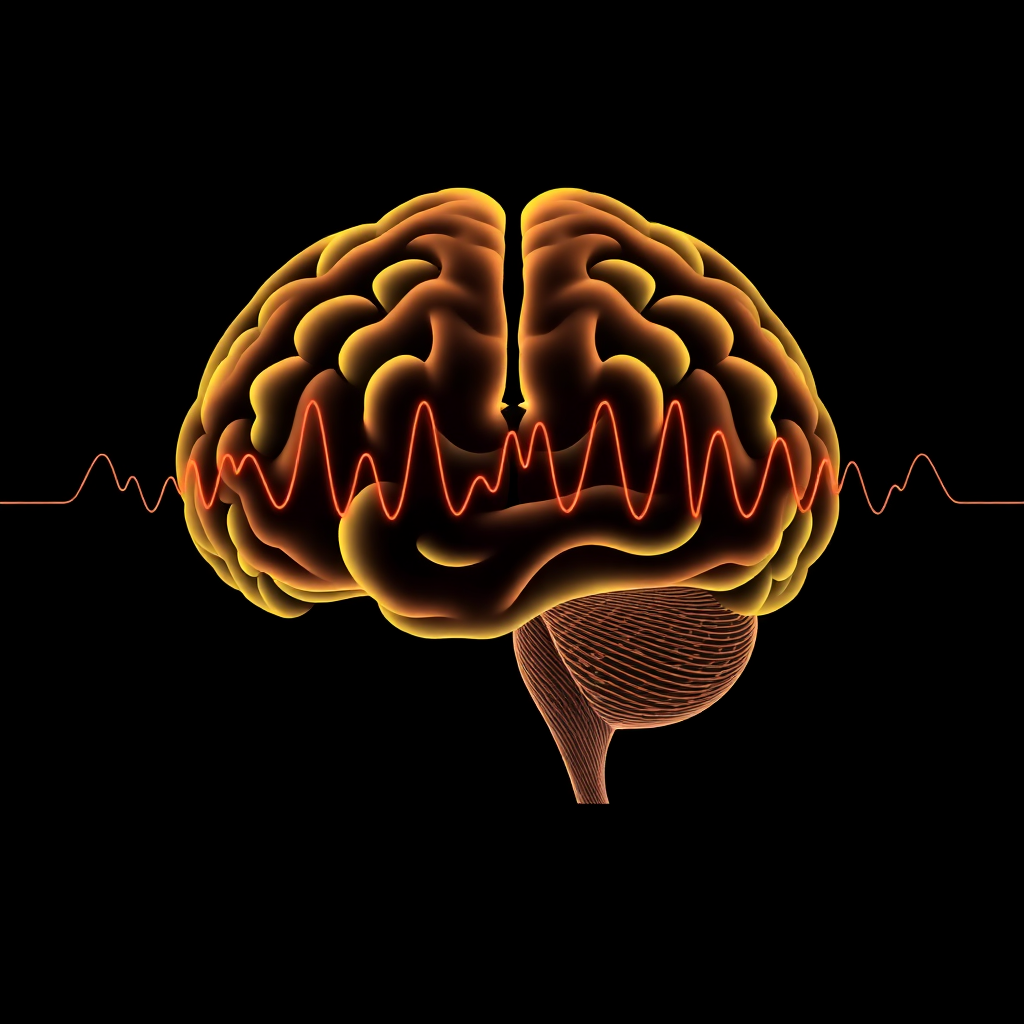
\includegraphics[width=0.8\textwidth]{images/brain_waves.png}

    \caption{Brain wave dynamics are essential for local conscious unification.}
\end{figure}

The role of electromagnetic fields in establishing and maintaining neural coherence finds substantial empirical support through recent neurobiological research \cite{Frohlich2010}. Studies have demonstrated how endogenous electric fields can guide neocortical network activity, suggesting that field effects play a crucial role in coordinating neural function. These findings provide important validation for both EM field theories and ECC's broader framework of energetic coherence.

The precise timing requirements of conscious processing raise important questions about mechanisms of neural synchronization \cite{Radman2007}. EM field theories suggest that electromagnetic fields provide a natural substrate for coordinating neural activity across different brain regions. This aligns with ECC's emphasis on how coherent energy states achieve temporal integration through physical rather than computational mechanisms.

Recent theoretical work has explored how information might be integrated in the brain's electromagnetic field \cite{McFadden2020}. While traditional approaches focus on synaptic connectivity, field theories suggest that EM fields provide an additional layer of integration that helps create unified conscious experience. This perspective complements ECC's broader framework of energetic coherence while suggesting specific mechanisms for its implementation.

The relationship between field effects and neural computation \cite{Weiss2010} reveals important questions about how physical and computational processes interact in conscious systems. Rather than treating computation and field effects as separate phenomena, EM field theories suggest they are intimately connected through the brain's electromagnetic dynamics. This aligns with ECC's view that conscious processing emerges from physical rather than purely computational mechanisms.

Experimental evidence has demonstrated how electric fields can amplify and coordinate neural activity \cite{Radman2007}. These findings suggest that field effects play a more fundamental role in neural processing than previously recognized. The ability of electromagnetic fields to influence spike timing and neural excitability provides crucial support for theories that emphasize the importance of field effects in consciousness.

The binding problem in consciousness studies \cite{Singer2001} finds potential resolution through field-based approaches. Rather than requiring computational mechanisms to bind different aspects of experience together, electromagnetic fields provide a natural substrate for integration. This aligns with ECC's emphasis on how coherent energy states achieve unity through physical rather than computational processes.

Recent developments in field theory approaches have emphasized how electromagnetic fields might contribute to both local and global aspects of conscious processing \cite{John2001}. The ability of fields to influence neural activity across multiple scales suggests they play a crucial role in creating the integrated yet differentiated character of conscious experience.

The question of how electromagnetic fields contribute to neural information processing remains an active area of investigation \cite{Barrett2011}. While some researchers emphasize the computational aspects of field effects, others focus on their role in coordinating and integrating neural activity. ECC suggests these perspectives might be unified by understanding how coherent energy states naturally support both information processing and integration through their physical dynamics.

Recent theoretical work has explored how electromagnetic fields might contribute to consciousness through their influence on neural timing and synchronization \cite{Pockett2012}. The ability of fields to coordinate activity across different neural populations suggests they play a crucial role in creating the temporal coherence characteristic of conscious experience. This aligns with ECC's emphasis on how physical mechanisms support conscious integration.

The relationship between attention and electromagnetic field effects \cite{Prinz2012} reveals important questions about conscious control mechanisms. While traditional approaches focus on synaptic mechanisms of attention, field theories suggest that electromagnetic fields might provide an additional layer of control over neural processing. This perspective complements ECC's broader framework while suggesting specific mechanisms for attentional modulation.

Empirical studies have demonstrated how electromagnetic fields shape morphogenesis and consciousness through environmental orchestration \cite{Rouleau2014}. These findings suggest that field effects play a fundamental role in both the development and ongoing function of conscious systems. This provides important support for theories that emphasize the importance of field effects in biological organization.

The integration of electromagnetic approaches with broader theories of consciousness \cite{McFadden2020} suggests productive new directions for research. By examining how field effects contribute to conscious processing while maintaining connection to other physical mechanisms, we may develop more sophisticated understanding of how consciousness emerges from biological systems.

These theoretical syntheses reveal important connections between electromagnetic field theories and other approaches to consciousness \cite{John2001}. While EM field theories provide crucial insights about specific physical mechanisms, ECC suggests these mechanisms operate within a broader framework of energetic coherence. This integration offers promising directions for future research into the physical basis of consciousness.

The future development of field-based approaches to consciousness will likely require sophisticated integration of theoretical insights with empirical investigation \cite{Singer2001}. By examining how electromagnetic fields contribute to conscious processing while maintaining connection to other physical mechanisms, we may develop increasingly sophisticated understanding of how consciousness emerges from biological systems.

In support of the EM Field view, recent research has significantly advanced our understanding of ephaptic coupling's role in neural information processing and potential contributions to consciousness. Evidence suggests that electric fields generated by neural activity can directly influence nearby neurons through non-synaptic mechanisms, creating a form of neural communication that operates alongside traditional synaptic transmission \cite{Pinotsis2023Ephaptic}. These field effects may contribute to the formation and stabilization of memory networks, suggesting a broader role for electromagnetic fields in neural information processing than previously recognized.

The concept of cytoelectric coupling has emerged as particularly significant, describing how electric fields can sculpt neural activity patterns and effectively "tune" the brain's infrastructure \cite{Pinotsis2023Cytoelectric}. Detailed modeling work has demonstrated that these ephaptic effects operate at the mesoscopic scale in human brain tissue, potentially contributing to neural synchronization and information integration \cite{Reimann2020Modeling}. Recent theoretical analysis suggests that ephaptic coupling may fundamentally contribute to brain complexity \cite{Cunha2024Ephapticity}, while studies of coincidence detector neurons in the auditory brainstem have revealed how endogenous electric fields can influence neural timing and synchronization \cite{Goldwyn2016Neuronal}. These findings align with ECC's emphasis on field effects in conscious processing, suggesting that ephaptic coupling might represent one mechanism through which the brain maintains the coherent energy states necessary for consciousness.

The role of ephaptic coupling in neural information processing suggests intriguing possibilities for how electromagnetic fields contribute to conscious experience. Beyond merely serving as a byproduct of neural activity, these fields may actively shape neural dynamics across multiple spatial scales. The ability of electric fields to modify neural timing and synchronization through ephaptic effects \cite{Goldwyn2016Neuronal} could provide a physical mechanism for the kind of rapid information integration that consciousness requires.

Research into memory network formation through ephaptic coupling \cite{Pinotsis2023Ephaptic} reveals how field effects might contribute to the stability of conscious states while allowing for dynamic reorganization. The concept of cytoelectric coupling \cite{Pinotsis2023Cytoelectric} suggests that electromagnetic fields play an active role in shaping neural architecture, potentially creating the conditions necessary for conscious processing through continuous field-mediated feedback between neurons and their environment.

Detailed modeling of mesoscopic ephaptic coupling in human brain tissue \cite{Reimann2020Modeling} has demonstrated that these effects operate at scales relevant for conscious integration. The contribution of ephaptic coupling to brain complexity \cite{Cunha2024Ephapticity} aligns with ECC's emphasis on consciousness requiring sophisticated patterns of energetic coherence. These findings suggest that ephaptic coupling might represent a crucial mechanism through which the brain achieves the field coherence necessary for conscious experience while maintaining the flexibility required for adaptive behavior.

This research indicates that electromagnetic fields in neural tissue serve not merely as epiphenomena but as active participants in neural information processing and conscious integration. The ability of ephaptic coupling to influence neural timing and synchronization without direct synaptic contact provides a potential physical basis for the kind of field-mediated integration that consciousness appears to require. These insights strengthen ECC's emphasis on field effects while suggesting specific mechanisms through which these fields might contribute to conscious experience.

\section{Basal Cognition}

Lynn Margulis' work on cellular consciousness and symbiogenesis, alongside recent research \cite{Lyon2015}, reveals that even simple cellular collectives demonstrate remarkable information processing capabilities through bioelectric signaling and membrane dynamics. Margulis' insight that consciousness has roots in bacterial awareness \cite{Margulis2001}, combined with contemporary findings \cite{Baluska2016}, suggests that the complex electromagnetic fields supporting consciousness in neural tissue represent an elaboration of primitive cellular communication mechanisms rather than a novel innovation.

The key insights from recent theoretical work show that cognitive-like processes—decision-making, memory, and pattern recognition—exist at the cellular level without requiring neurons or synapses \cite{Shapiro2007}. These capabilities depend critically on bioelectric fields and membrane potentials, the same physical phenomena that, at a more complex level, contribute to conscious processing in neural tissue. Research on bacterial consciousness \cite{vanDuijn2006} and bioelectric fields suggests consciousness emerged through the progressive refinement and integration of basic cellular awareness mechanisms rather than appearing suddenly with neural complexity.

Recent work \cite{Lane2015} complements these perspectives by emphasizing how membrane dynamics and ion gradients form the basis of all biological information processing. The ability to maintain ion gradients across membranes represents one of life's fundamental innovations, enabling both energy storage and information processing. This dual role of membranes—as both energetic and informational structures—aligns with both cellular approaches to consciousness and ECC's emphasis on the inseparability of energy dynamics and conscious processing.

Contemporary research on basal cognition \cite{Levin2019} demonstrates that cognitive capabilities emerge from fundamental cellular processes. These findings suggest consciousness evolved not merely through increasing neural complexity but through the progressive elaboration of basic cellular awareness mechanisms that were present from life's earliest stages. The convergence of these perspectives provides strong support for ECC's emphasis on energetic coherence as fundamental to consciousness.

Theoretical developments in understanding biological computation \cite{Levin2018} suggest a deeper physical basis for conscious processing. The electromagnetic fields that help sustain conscious states through neural light cones may represent a sophisticated elaboration of more basic bioelectric fields present in all cells. The complex interference patterns possible in neural tissue might have evolved from simpler patterns of membrane potential coordination in cellular collectives.

The rich alphabet that ECC posits as necessary for consciousness—implemented through transcriptomic profiles and protein configurations—may have its origins in the diverse membrane proteins and ion channels that enable basic cellular cognition \cite{Fields2020}. This suggests a continuity between basal cellular information processing and conscious experience that helps explain how consciousness could have emerged through evolution.

Recent work on biological decision-making \cite{Mitchell2016} demonstrates how even simple cellular systems achieve sophisticated information processing through molecular mechanisms. These findings support the idea that consciousness represents an elaboration of fundamental biological capabilities rather than a completely novel emergence.

The relationship between basal cognition and membrane dynamics becomes even richer when considering the role of genetic regulation \cite{Manicka2019}. DNA can be understood as providing metaprograms that shape cellular behavior across different timescales, while RNA serves as more immediate programs that fine-tune cellular responses through transcriptomic profiles. This hierarchical regulatory system fundamentally shapes both basal cognition and membrane dynamics.

The cognitive capabilities of cellular systems \cite{Lyon2015} demonstrate sophisticated information processing without requiring neural architecture. Recent work has shown how cells achieve complex computational tasks through membrane dynamics and bioelectric signaling \cite{Levin2018}. These findings suggest that consciousness builds upon fundamental cellular mechanisms rather than emerging solely from neural complexity.

Research on bacterial cognition \cite{Shapiro2007} reveals remarkable decision-making capabilities in simple organisms. These studies demonstrate how basic cellular processes support sophisticated information processing through membrane dynamics and molecular signaling. The cognitive capabilities of bacteria suggest that consciousness represents an elaboration of fundamental biological mechanisms rather than a novel emergence.

The physical basis of biological computation \cite{Pattee2001} takes on particular significance when examining basal cognition. Rather than implementing abstract computational processes, cellular systems achieve information processing through concrete physical mechanisms involving membrane dynamics and molecular interactions. This aligns with ECC's emphasis on how consciousness emerges from physical rather than purely computational processes.

Recent theoretical work \cite{Fields2020} has emphasized how scale-free principles operate across biological systems. The same fundamental mechanisms that enable cellular cognition may scale up to support more complex forms of consciousness through progressive elaboration and integration. This suggests important continuities between basic cellular processing and conscious experience.

The role of bioelectric fields in morphogenesis and cognition \cite{Levin2019} provides crucial insight into how cellular mechanisms support information processing. These fields coordinate cellular behavior across multiple scales, suggesting how simple awareness mechanisms might have evolved into more complex forms of consciousness. The ability of bioelectric fields to influence both development and cognition reveals important connections between cellular and neural processing.

Studies of minimal cognition in simple organisms \cite{vanDuijn2006} demonstrate how basic biological mechanisms support sophisticated information processing. These findings suggest that consciousness emerges from fundamental cellular capabilities rather than requiring entirely new mechanisms. The cognitive abilities of simple organisms provide important insight into how consciousness might have evolved from basic cellular processes.

The relationship between cellular and conscious information processing \cite{Margulis2001} gains new significance when examined through modern theoretical frameworks. Recent studies of basal cognition \cite{Levin2018} demonstrate how fundamental cellular mechanisms achieve sophisticated computation through physical rather than abstract processes. This suggests consciousness represents an elaboration of basic biological capabilities rather than a wholly novel phenomenon.

The computational boundary of biological systems \cite{Levin2019} reveals important questions about how information processing scales across different levels of organization. While traditional approaches often treat computation as abstract symbol manipulation, research on cellular cognition suggests that biological information processing emerges from concrete physical mechanisms. This aligns with ECC's emphasis on how consciousness arises from actual physical dynamics rather than purely computational processes.

Studies of cognitive cell biology \cite{Mitchell2016} have demonstrated how cellular decisions emerge from complex molecular interactions. Rather than implementing abstract algorithms, cells achieve sophisticated information processing through the physical dynamics of membrane potentials and molecular signaling. These findings suggest important continuities between cellular cognition and conscious processing.

Recent theoretical developments \cite{Fields2020} emphasize how biological computation operates across multiple scales through consistent principles. The same mechanisms that enable cellular decision-making may support more complex forms of consciousness through progressive elaboration and integration. This suggests consciousness represents an extension of fundamental biological capabilities rather than requiring entirely new mechanisms.

The role of molecular communication in cellular cognition \cite{Manicka2019} provides crucial insight into how biological systems achieve information processing. Rather than implementing abstract computation, cells process information through concrete physical mechanisms involving membrane dynamics and molecular interactions. This aligns with ECC's emphasis on how consciousness emerges from actual physical processes.

These theoretical syntheses suggest productive new directions for consciousness research that examine how basic cellular mechanisms support increasingly sophisticated forms of awareness \cite{Baluska2016}. By understanding how consciousness emerges from fundamental biological processes, we may develop more sophisticated theories that bridge cellular and neural approaches to mind while maintaining closer contact with physical reality.

The future investigation of consciousness may require careful examination of how basic cellular mechanisms elaborate into more complex forms of awareness \cite{Lyon2015}. This suggests new experimental approaches that examine consciousness across multiple scales of biological organization while maintaining connection to fundamental physical processes.

\section{Quantum Theories}

The Penrose-Hameroff Orchestrated Objective Reduction (Orch OR) theory \cite{Hameroff2014} represents perhaps the most developed quantum theory of consciousness, proposing that quantum computations in microtubules give rise to conscious experience. While ECC does not depend on quantum effects for its core mechanisms, certain aspects of quantum physics might influence the electromagnetic fields that help sustain conscious states.

Early work exploring quantum aspects of brain activity \cite{Beck1992} suggested potential roles for quantum mechanics in neural processing. However, ECC maintains that classical electromagnetic fields and molecular dynamics provide sufficient basis for understanding conscious processing. The complex interference patterns possible in neural tissue, combined with the rich alphabet of protein states and membrane dynamics, may not require quantum effects to explain conscious experience.

Critical analysis of quantum approaches \cite{Tegmark2000} has raised important questions about the feasibility of maintaining quantum coherence in the warm, wet environment of the brain. ECC aligns with this perspective, suggesting that consciousness emerges from classical field dynamics that operate at scales above quantum decoherence thresholds. This classical approach aligns with the thermodynamic constraints observed in biological systems.

The philosophical implications of quantum consciousness theories \cite{Stapp2009} raise fundamental questions about the relationship between mind and matter. While quantum theories often suggest consciousness requires quantum effects, ECC proposes that classical field dynamics provide sufficient basis for understanding how consciousness emerges from physical systems. This maintains closer connection to established biological mechanisms while avoiding speculative quantum requirements.

Recent theoretical developments \cite{Hagan2002} have attempted to address the decoherence challenge by proposing specific mechanisms for maintaining quantum coherence in biological systems. However, ECC suggests that even if quantum effects play some role in neural processing, consciousness itself emerges from classical patterns of energetic coherence that operate at larger scales.

Early philosophical work on quantum mechanics and consciousness \cite{Bohm1990} proposed deep connections between quantum processes and mental phenomena. While these perspectives raise important questions about the nature of consciousness, ECC suggests that understanding conscious experience requires examining classical field dynamics rather than quantum effects.

The relationship between quantum mechanics and brain function \cite{Koch2006} remains a matter of ongoing investigation. While quantum effects might influence certain aspects of neural processing, ECC proposes that consciousness emerges from classical patterns of energetic coherence that can be understood without invoking quantum mechanisms.

Although Penrose's early proposals \cite{Penrose1989, Penrose1994} suggested fundamental connections between quantum processes and consciousness, ECC suggests that classical field dynamics provide a more plausible physical basis for conscious experience. While quantum effects might operate at microscopic scales, the coherent energy patterns that support consciousness likely emerge from classical mechanisms operating at larger scales.

Detailed physical analysis \cite{Tegmark2000} has demonstrated significant challenges for quantum consciousness theories, particularly regarding decoherence timescales in biological systems. The brain operates at temperatures and scales where quantum coherence is difficult to maintain, though quantum effects might still influence field dynamics through more subtle mechanisms, including:

The mathematical frameworks developed for quantum consciousness \cite{Hagan2002} have contributed valuable insights about potential physical mechanisms of consciousness. However, ECC suggests that understanding consciousness requires examining classical field dynamics rather than quantum effects, while acknowledging that quantum properties might influence these classical fields in subtle ways.

Recent work on quantum biology \cite{Koch2006} has revealed quantum effects in certain biological processes, such as photosynthesis and magnetic sensing. While these findings demonstrate that quantum mechanisms can operate in biological systems, ECC maintains that consciousness itself likely emerges from classical patterns of energetic coherence rather than requiring quantum computation.

The relationship between quantum mechanics and brain function \cite{Stapp2009} raises important questions about causation and measurement in conscious systems. While quantum theories often invoke measurement problems to explain consciousness, ECC suggests that conscious experience emerges from classical field dynamics that can be understood without reference to quantum measurement paradoxes.

The original proposals linking quantum mechanics to consciousness \cite{Beck1992} highlighted important questions about the physical basis of mental phenomena. However, ECC suggests that understanding consciousness requires examining classical field dynamics rather than quantum effects, while maintaining the possibility that quantum properties might influence these classical patterns in subtle ways.

Recent theoretical developments \cite{Hameroff2014} have attempted to address criticisms of quantum consciousness theories by proposing specific mechanisms for maintaining quantum coherence. However, ECC suggests that even if such mechanisms exist, consciousness itself likely emerges from classical patterns of energetic coherence operating at scales above quantum decoherence thresholds.

The microtubule hypothesis central to quantum theories \cite{Hameroff2014} raises important questions about cellular organization in consciousness. While ECC acknowledges the importance of microtubules in cellular function, it suggests their role emerges through classical rather than quantum mechanisms. From a purely classical perspective, microtubules serve as crucial integrative structures that, like membranes, play essential roles in both information processing and mechanical output.

Building on foundational quantum approaches \cite{Penrose1989}, recent work has explored potential quantum effects in neural systems. However, ECC suggests that understanding consciousness requires examining classical field dynamics that operate at scales where quantum coherence is unlikely to persist. This aligns with critical analyses \cite{Tegmark2000} demonstrating the challenges of maintaining quantum states in biological systems.

The philosophical implications of quantum consciousness theories \cite{Bohm1990} extend beyond purely physical considerations. While these approaches often suggest deep connections between quantum mechanics and mind, ECC proposes that conscious experience emerges from classical patterns of energetic coherence that can be understood without invoking quantum effects.

Contemporary research on quantum biology \cite{Koch2006} has revealed quantum effects in specific biological processes. However, ECC maintains that consciousness itself likely emerges from classical mechanisms, even if quantum effects influence certain aspects of cellular function. This perspective aligns with empirical evidence about the scales at which conscious processing occurs.

The relationship between quantum mechanics and consciousness \cite{Stapp2009} remains contentious within neuroscience. While quantum theories offer intriguing possibilities, ECC suggests that understanding consciousness requires examining classical field dynamics that operate at scales where quantum effects are unlikely to play a direct role.

These theoretical syntheses suggest productive new directions for consciousness research that examine both classical and quantum mechanisms \cite{Hagan2002}. By understanding how different physical processes contribute to conscious experience across multiple scales, we may develop more sophisticated theories that bridge quantum and classical approaches while maintaining closer contact with biological reality.

The future investigation of consciousness will likely require careful examination of how different physical mechanisms interact across scales \cite{Beck1992}. This suggests new experimental approaches that examine consciousness at multiple levels of organization while maintaining connection to fundamental physical processes.

\section{Embodied Consciousness}

The relationship between consciousness and embodiment has been extensively explored in foundational work \cite{Varela1991, MerleauPonty1962} that emphasizes how conscious experience emerges from the dynamic coupling between organism and environment. Where traditional cognitive science often treats the body as merely an input-output system for an abstract mind, both phenomenological approaches and ECC emphasize how consciousness emerges from the concrete dynamics of biological organization.

Recent theoretical developments \cite{Thompson2007} have emphasized how consciousness cannot be understood in isolation from the physical body and its environmental interactions. This perspective resonates with ECC's framework in several important ways, particularly regarding how patterns of energetic coherence emerge from and support embodied activity. The framework suggests that consciousness requires specific forms of physical organization that cannot be reduced to computational representation.

Early phenomenological insights \cite{MerleauPonty1962} about the primacy of embodied perception anticipated many contemporary developments in consciousness studies. The concept of the "body schema" - our implicit understanding of our body's capabilities and position - can be understood through ECC as emerging from patterns of energetic coherence that span brain and body rather than abstract representation.

Contemporary work on embodied cognition \cite{Clark1997} has demonstrated how consciousness emerges from the dynamic interaction between organism and environment. While some approaches attempt to reduce embodiment to computational models, ECC reveals how consciousness emerges from actual patterns of energetic coherence that cannot be adequately captured through computational representation.

The philosophical foundations of embodied consciousness \cite{Lakoff1999} emphasize how mental processes are fundamentally shaped by physical embodiment. ECC strengthens this position by demonstrating how consciousness emerges from specific patterns of energetic coherence maintained through biological systems, rather than from abstract computation alone.

Research on skilled action and embodied knowledge \cite{Ingold2000} reveals how consciousness emerges from practical engagement with the environment. Rather than treating bodily processes as inputs to be modeled, ECC shows how consciousness is inherently embodied through its physical emergence from coherent energy dynamics.

Anthropological perspectives on embodiment \cite{Csordas1994} have emphasized how conscious experience is shaped by cultural and physical practices. ECC provides a physical framework for understanding how these embodied practices influence consciousness through their effects on patterns of energetic coherence.

The anticomputationalist stance developed in seminal work \cite{Dreyfus1992} finds support in ECC's demonstration that consciousness requires specific forms of physical organization that cannot be reduced to computation. This perspective challenges attempts to reduce embodied cognition to computational representations of bodily states, suggesting instead that consciousness emerges from actual physical dynamics.

Recent research on the relationship between body and mind \cite{Gallagher2005} has revealed how consciousness emerges from embodied activity rather than abstract mental processes. ECC extends this insight by showing how patterns of energetic coherence necessarily span both brain and body, creating an integrated field of conscious experience that cannot be reduced to purely neural computation.

The phenomenology of bodily experience \cite{Leder1990} takes on new significance when examined through ECC's framework. Rather than treating bodily awareness as a form of internal representation, ECC suggests that conscious bodily experience emerges directly from patterns of energetic coherence that naturally span neural and bodily tissues.

Contemporary work on perception and action \cite{Noe2004} emphasizes how conscious experience emerges from active engagement with the environment. ECC provides a physical basis for understanding this relationship, showing how patterns of energetic coherence naturally support both perception and action through their embodied dynamics.

Theoretical developments in embodied cognition \cite{Thompson2007} have demonstrated how consciousness requires ongoing interaction between organism and environment. Rather than treating this interaction as computational input-output, ECC reveals how conscious experience emerges from continuous patterns of energetic coherence that span brain, body, and environment.

Anthropological studies of skilled practice \cite{Marchand2010} show how consciousness emerges from embodied engagement with the world. ECC provides a physical framework for understanding how these practices shape consciousness through their effects on patterns of energetic coherence rather than through abstract representation.

Studies of sensory experience \cite{Howes2003} reveal how consciousness emerges from multiple forms of bodily engagement with the environment. ECC suggests that this multisensory integration occurs through patterns of energetic coherence that naturally span different sensory modalities rather than requiring computational binding mechanisms.

The relationship between embodiment and conscious experience \cite{Jackson1989} gains new significance when examined through ECC's framework. Rather than treating embodiment as an implementation detail, ECC reveals how consciousness necessarily emerges from specific patterns of energetic coherence that span brain and body, making embodiment essential rather than incidental to conscious experience.

Recent work on the philosophical implications of embodiment \cite{Lakoff1999} aligns with ECC's demonstration that consciousness cannot be reduced to abstract computation. The framework shows how conscious experience requires actual physical dynamics that emerge from biological organization rather than computational representation of bodily states.

The ecological approach to perception \cite{Gibson1979} finds natural extension through ECC's emphasis on how consciousness emerges from organism-environment interaction. Rather than treating perception as internal representation, ECC shows how perceptual experience emerges from patterns of energetic coherence that naturally span perceiver and environment.

Studies of skilled bodily practice \cite{Ingold2000} reveal how consciousness emerges from embodied engagement with the world. ECC provides a physical framework for understanding how these practices shape consciousness through their effects on patterns of energetic coherence rather than through abstract mental representations.

Contemporary research on embodied cognition \cite{Clark1997} demonstrates how consciousness requires ongoing interaction between organism and environment. ECC extends this insight by showing how patterns of energetic coherence necessarily span brain, body, and environment, creating an integrated field of conscious experience.

Phenomenological investigations \cite{MerleauPonty1962} have long emphasized the primacy of embodied experience. ECC provides physical mechanisms that explain how consciousness emerges from embodied dynamics, supporting phenomenological insights while grounding them in concrete physical processes.

These theoretical syntheses suggest new directions for investigating how consciousness emerges from embodied activity \cite{Varela1991}. By examining how patterns of energetic coherence span brain, body, and environment, we may develop more sophisticated understanding of consciousness while maintaining closer contact with physical reality.

\newpage
\section{References}
\printbibliography[title={},heading=subbibliography]
%\printbibliography[title={Comparative Analysis: Embodied Consciousness}]
\end{refsection}